\documentclass[11pt,fleqn,oneside]{book} % Default font size and left-justified equations

% COMPILES THE COVER IF 1 
% DOESN'T COMPILE THE COVER IF 0
\newcommand{\showCover}{0} 

\usepackage{fontawesome5}

% =========================================================
% Global settings
\newcommand{\AUTHOR}{Federico Brancasi}
\newcommand{\CLIENT}{Client Name}
\newcommand{\DATE}{\today}
% \newcommand{\VERSION}{1.0.0}
\newcommand{\TITLE}{Deep Learning}
\newcommand{\SUBTITLE}{University of Trento}
\newcommand{\SUBJECT}{Demo}
% \newcommand{\URL}{https://github.com/federicobrancasi}

%%%%%%%%%%%%%%%%%%%%%%%%%%%%%%%%%%%%%%%%%
% By Apehex
% github.com/apehex
%
% Built upon the The Legrand Orange Book by:
% Mathias Legrand (legrand.mathias@gmail.com)
%
% License:
% CC BY-NC-SA 3.0 (http://creativecommons.org/licenses/by-nc-sa/3.0/)
%
%%%%%%%%%%%%%%%%%%%%%%%%%%%%%%%%%%%%%%%%%

%------------------------------------------------------------------------------
%   GENERIC
%------------------------------------------------------------------------------

% ALL GENERIC FEATURES --------------------------------------------------------
%%%%%%%%%%%%%%%%%%%%%%%%%%%%%%%%%%%%%%%%%
% By Apehex
% github.com/apehex
%
% Built upon the The Legrand Orange Book by:
% Mathias Legrand (legrand.mathias@gmail.com)
%
% License:
% CC BY-NC-SA 3.0 (http://creativecommons.org/licenses/by-nc-sa/3.0/)
%
%%%%%%%%%%%%%%%%%%%%%%%%%%%%%%%%%%%%%%%%%

%------------------------------------------------------------------------------
%   GENERIC
%------------------------------------------------------------------------------

% THEMES ----------------------------------------------------------------------
%----------------------------------------------------------------------------------------
%   SOLVE CONFLICTS
%----------------------------------------------------------------------------------------
\PassOptionsToPackage{table}{xcolor}

%----------------------------------------------------------------------------------------
%   COLORS
%----------------------------------------------------------------------------------------
\usepackage[table, usenames,dvipsnames]{xcolor} % Required for specifying colors by name
\usepackage{pagecolor} % dark theme

\colorlet{myred}{red!80!black}
\colorlet{myblue}{blue!80!black}
\colorlet{mybluee}{myblue!80!black}
\colorlet{mygreen}{green!60!black}
\colorlet{myorange}{orange!70!red!60!black}
\colorlet{mydarkred}{red!30!black}
\colorlet{mydarkblue}{blue!40!black}
\colorlet{mydarkgreen}{green!30!black}

%----------------------------------------------------------------------------------------
%   MAKE BOLD STAND OUT
%----------------------------------------------------------------------------------------
\let\oldtextbf\textbf

%----------------------------------------------------------------------------------------
%   DARK THEME
%----------------------------------------------------------------------------------------
\newcommand{\togglethemedark}{
%----------------------------------------------------------------------------------------
\colorlet{accent}{orange}
\colorlet{fg}{white}
\colorlet{fgalt}{lightgray}
\colorlet{fgacc}{white}
\colorlet{bg}{black}
\colorlet{bgalt}{darkgray}
\colorlet{bgacc}{orange}
\colorlet{border}{white}
\colorlet{borderalt}{lightgray}
\colorlet{borderacc}{orange}
%----------------------------------------------------------------------------------------
\pagecolor{bg}
\color{fgalt}
\renewcommand{\textbf}[1]{\oldtextbf{\color{fg}##1}}
}

%----------------------------------------------------------------------------------------
%   LIGHT THEME
%----------------------------------------------------------------------------------------
\newcommand{\togglethemelight}{
%----------------------------------------------------------------------------------------
\colorlet{accent}{orange}
\colorlet{fg}{black}
\colorlet{fgalt}{darkgray}
\colorlet{fgacc}{black}
\colorlet{bg}{white}
\colorlet{bgalt}{lightgray}
\colorlet{bgacc}{orange}
\colorlet{border}{black}
\colorlet{borderalt}{darkgray}
\colorlet{borderacc}{orange}
%----------------------------------------------------------------------------------------
\pagecolor{bg}
\color{fgalt}
\renewcommand{\textbf}[1]{\oldtextbf{\color{fg}##1}}
}

%----------------------------------------------------------------------------------------
%   FORTA THEME
%----------------------------------------------------------------------------------------
\newcommand{\togglethemeforta}{
%----------------------------------------------------------------------------------------
\colorlet{accent}{white}
\colorlet{fg}{white}
\colorlet{fgalt}{lightgray}
\colorlet{fgacc}{black}
\colorlet{bg}{black}
\colorlet{bgalt}{darkgray}
\colorlet{bgacc}{white}
\colorlet{border}{white}
\colorlet{borderalt}{lightgray}
\colorlet{borderacc}{white}
%----------------------------------------------------------------------------------------
\pagecolor{bg}
\color{fgalt}
\renewcommand{\textbf}[1]{\oldtextbf{\color{fg}##1}}
}


%----------------------------------------------------------------------------------------
%   DL THEME
%----------------------------------------------------------------------------------------
\newcommand{\togglethemedl}{
%----------------------------------------------------------------------------------------
\colorlet{accent}{black}
\colorlet{fg}{black}
\colorlet{fgalt}{darkgray}
\colorlet{fgacc}{white}
\colorlet{bg}{white}
\colorlet{bgalt}{lightgray}
\colorlet{bgacc}{black}
\colorlet{border}{black}
\colorlet{borderalt}{darkgray}
\colorlet{borderacc}{black}
%----------------------------------------------------------------------------------------
\pagecolor{bg}
\color{fgalt}
\renewcommand{\textbf}[1]{\oldtextbf{\color{fg}##1}}
}

\togglethemedl

% GEOMETRY --------------------------------------------------------------------
\usepackage{calc} % coordinate calculations

% PAGE LAYOUT -----------------------------------------------------------------
%----------------------------------------------------------------------------------------
%   PARAGRAPH FORMATING
%----------------------------------------------------------------------------------------

\setlength{\parindent}{0pt}
\setlength{\parskip}{12pt}

%----------------------------------------------------------------------------------------
%   FLOAT LAYOUT
%----------------------------------------------------------------------------------------

\renewcommand{\topfraction}{0.9}    % max fraction of floats at top
\renewcommand{\bottomfraction}{0.8} % max fraction of floats at bottom

%   Parameters for TEXT pages (not float pages):
\setcounter{topnumber}{2}
\setcounter{bottomnumber}{2}
\setcounter{totalnumber}{8}     % 2 may work better
\setcounter{dbltopnumber}{2}    % for 2-column pages
\renewcommand{\dbltopfraction}{0.9} % fit big float above 2-col. text
\renewcommand{\textfraction}{0.07}  % allow minimal text w. figs

%   Parameters for FLOAT pages (not text pages):
\renewcommand{\floatpagefraction}{0.7}  % require fuller float pages
\renewcommand{\dblfloatpagefraction}{0.7}   % require fuller float pages

% FONTS -----------------------------------------------------------------------
\usepackage{fontspec} % import new fonts
\usepackage[english]{babel}

%----------------------------------------------------------------------------------------
%   SPACING
%----------------------------------------------------------------------------------------

\usepackage{microtype}

%----------------------------------------------------------------------------------------
%   ADD BOLD + ITALIC
%----------------------------------------------------------------------------------------

\newfontfamily\inconsolatafontfamily[
    Path=template/generic/fonts/inconsolata/,
    Ligatures=TeX,
    Scale=MatchUppercase,
    UprightFont = *.otf,
    BoldFont = *-Bold.otf,
    ItalicFont = *-Italic.otf,
    BoldItalicFont = *-BoldItalic.otf
]{Inconsolata-LGC}

%----------------------------------------------------------------------------------------
%   FAMILY DEFAULTS
%----------------------------------------------------------------------------------------

% \setmonofont{\inconsolatafontfamily}
% \renewcommand*{\familydefault}{\ttdefault}

%----------------------------------------------------------------------------------------
%   HEADINGS
%----------------------------------------------------------------------------------------

\let\headingfontfamily\inconsolatafontfamily

% TITLES ----------------------------------------------------------------------
\usepackage{titlesec}

%----------------------------------------------------------------------------------------
%   SECTION NUMBERING IN THE MARGIN
%----------------------------------------------------------------------------------------

\newcommand{\autodot}{.} % separate title numbers with dots
\newcommand*{\numberinmargin}[3]{\makebox[0pt][r]{\textcolor{#3}{\fontsize{#2}{#2}\selectfont\headingfontfamily\bfseries\selectfont#1\autodot}\hskip\marginparsep}}

%----------------------------------------------------------------------------------------
%   LAYOUT
%----------------------------------------------------------------------------------------

\titlespacing*{\chapter}{0pt}{-30pt}{20pt}

\titlespacing*{\paragraph}{0pt}{3.25ex plus 1ex minus .2ex}{1.5ex plus .2ex}

%----------------------------------------------------------------------------------------
%   FORMAT
%----------------------------------------------------------------------------------------

\titleformat{\chapter}[hang]
  {\normalfont\huge\headingfontfamily\bfseries\selectfont\color{accent}}
  {\numberinmargin{\thechapter}{24}{accent}}
  {0pt}
  {\MakeUppercase}

\titleformat{\section}
  {\normalfont\large\headingfontfamily\bfseries\selectfont\color{fg}}
  {\numberinmargin{\thesection}{16}{accent}}
  {0pt}
  {\MakeUppercase}

\titleformat{\subsection}
  {\normalfont\normalsize\headingfontfamily\bfseries\selectfont\color{fg}}
  {\numberinmargin{\thesubsection}{12}{fg}}
  {0pt}
  {}

\titleformat{\subsubsection}
  {\normalfont\small\headingfontfamily\bfseries\selectfont\color{fg}}
  {\numberinmargin{\thesubsubsection}{10}{fg}}
  {0pt}
  {}

%----------------------------------------------------------------------------------------
%   SPECIAL TITLE
%----------------------------------------------------------------------------------------

\renewcommand{\paragraph}[1]{%
  \par\vspace{3.25ex plus 1ex minus .2ex}%
  \noindent\hspace*{-4cm}\colorbox{bgacc}{%
    \hspace*{4cm}\normalfont\huge\headingfontfamily\selectfont\color{fgacc}\uppercase{#1}
  }%
  \par\nobreak\vspace{1.5ex plus .2ex}%
}

% MATH ------------------------------------------------------------------------
\usepackage{amsmath,amsfonts,amssymb,amsthm} % For math equations, theorems, symbols, etc

\usepackage{tikz}
\usetikzlibrary{calc}
\newcommand{\tikzmarkk}[1]{\tikz[baseline,remember picture] \coordinate (#1) {};}

\usepackage{algorithm}
\usepackage{algorithmic}

% \usepackage{nccmath}
% LINKS -----------------------------------------------------------------------
\usepackage{hyperref}
\usepackage{bookmark}
\usepackage[all]{hypcap} % moves the ref jumping points to the top of images (instead of the caption)

%----------------------------------------------------------------------------------------
%   HYPERLINKS IN THE DOCUMENTS
%----------------------------------------------------------------------------------------
\hypersetup{
hidelinks,
% backref=true,
% pagebackref=true,
% hyperindex=true,
colorlinks=true,
breaklinks=true,
urlcolor=accent,
% bookmarks=true,
bookmarksopen=false,
pdftitle={\TITLE},
pdfauthor={\AUTHOR},
pdfsubject={\texorpdfstring{\SUBJECT}{}},
}

\bookmarksetup{
open,
numbered,
addtohook={%
\ifnum\bookmarkget{level}=0 % chapter
\bookmarksetup{bold}%
\fi
\ifnum\bookmarkget{level}=-1 % part
\bookmarksetup{color=accent,bold}%
\fi
}
}

%----------------------------------------------------------------------------------------
%   BOLD HREF
%----------------------------------------------------------------------------------------

\let\oldhref\href
\renewcommand{\href}[2]{\oldhref{#1}{\headingfontfamily\textbf{#2}}}

% LISTS -----------------------------------------------------------------------
\usepackage{enumitem} % Customize lists

%----------------------------------------------------------------------------------------
%   BULLET POINTS
%----------------------------------------------------------------------------------------

\setlist{nolistsep} % Reduce spacing between bullet points and numbered lists
\setlist[itemize]{leftmargin=4mm}
\setlist[enumerate]{leftmargin=4mm}

%----------------------------------------------------------------------------------------
%   DESCRIPTIONS
%----------------------------------------------------------------------------------------

% \newlength{\desclabelwidth}
% \setlength{\desclabelwidth}{4cm} % default value

% \renewenvironment{description}[1][4cm]
% {\setlength{\desclabelwidth}{#1}
% \begin{list}{}{
%     \renewcommand*{\makelabel}[1]{\bfseries##1\hspace{\desclabelwidth}}
%     \setlength{\itemsep}{0pt}
%     \setlength{\parsep}{0pt}
%     \setlength{\labelsep}{0pt}
%     \setlength{\leftmargin}{0pt}
%     \setlength{\itemindent}{\desclabelwidth}}}
% {\end{list}}

% CODE ------------------------------------------------------------------------
\usepackage{listings}

\input{template/generic/syntax/solidity}

% HEADERS ---------------------------------------------------------------------
\usepackage{fancyhdr} % Required for header and footer configuration

%----------------------------------------------------------------------------------------
%   PAGE HEADERS
%----------------------------------------------------------------------------------------

\fancypagestyle{plain}{%
    % Clear all headers and footers
    \fancyhf{}

    % Remove horizontal line in the header
    \renewcommand{\headrulewidth}{0pt}

    % Page number centered at the bottom
    \fancyfoot[C]{\thepage}
}

\fancypagestyle{fancy}{%
    % Clear all headers and footers
    \fancyhf{}

    % Remove horizontal line in the header
    \renewcommand{\headrulewidth}{0pt}

    % Page number centered at the bottom
    \fancyfoot[C]{\thepage}
}

% BOXES -----------------------------------------------------------------------
\usepackage[most]{tcolorbox}

%----------------------------------------------------------------------------------------
%   HIGHLIGHT ENVIRONMENT
%----------------------------------------------------------------------------------------

\newtcolorbox{highlight}{
  colback=bg,
  colframe=accent,
  coltext=fg,
  boxrule=2pt,
  boxsep=4pt,
  arc=0pt,
  outer arc=0pt
}

%----------------------------------------------------------------------------------------
%   REMARK ENVIRONMENT
%----------------------------------------------------------------------------------------

\newtcolorbox{remark}{
  colback=bg,
  colframe=accent,
  coltext=fg,
  boxrule=0pt,
  leftrule=2pt,
  boxsep=4pt,
  arc=0pt,
  outer arc=0pt,
}

%----------------------------------------------------------------------------------------
%   OUTLINE ENVIRONMENT
%----------------------------------------------------------------------------------------

\newtcolorbox{outline}[1][4pt]{
  enhanced,
  colback=bg,
  colframe=bg, % To essentially hide the frame, but we will draw the corners manually
  coltext=fg,
  boxrule=0pt,
  boxsep=#1,
  arc=0pt,
  outer arc=0pt,
  overlay={
    % Top left corner
    \draw[accent,line width=2pt] 
      (frame.north west) -- ++(0,-0.25*\tcbtextheight)
      (frame.north west) -- ++(0.25*\tcbtextwidth,0);
    % Bottom right corner
    \draw[accent,line width=2pt]
      (frame.south east) -- ++(0,0.25*\tcbtextheight)
      (frame.south east) -- ++(-0.25*\tcbtextwidth,0);
  }
}

% CAPTIONS --------------------------------------------------------------------
\usepackage{caption}

%----------------------------------------------------------------------------------------
%   COMMON
%----------------------------------------------------------------------------------------

\DeclareCaptionFont{fg}{\color{fg}}
\DeclareCaptionFont{accent}{\color{accent}}

%----------------------------------------------------------------------------------------
%   CODE: LSTLISTING
%----------------------------------------------------------------------------------------

\DeclareCaptionFormat{listing}{\colorbox{border}{\parbox{\dimexpr\linewidth-2\fboxsep\relax}{#1#2#3}}}
\captionsetup[lstlisting]{
  format=listing,
  labelfont=accent,
  textfont=fg,
  labelformat=empty,
  listformat=empty,
  singlelinecheck=false,
  margin=0pt,
  font={bf,footnotesize}
}

%----------------------------------------------------------------------------------------
%   TABLES
%----------------------------------------------------------------------------------------

\captionsetup[table]{
  labelformat=empty,
  listformat=empty,
}

%----------------------------------------------------------------------------------------
%   FIGURES
%----------------------------------------------------------------------------------------

\captionsetup[figure]{
  labelformat=empty,
  listformat=empty,
}

% ILLUSTRATIONS ---------------------------------------------------------------
\usepackage{graphicx} % Required for including pictures
\graphicspath{{images/}} % Specifies the directory where pictures are stored

\usepackage{tikz} % Required for drawing custom shapes
\usetikzlibrary{arrows, backgrounds, calc, fit, math, mindmap, positioning, shapes, shapes.geometric, tikzmark}

%----------------------------------------------------------------------------------------
%   GEOMETRY
%----------------------------------------------------------------------------------------

\newcommand{\drawhexagon}[5]{
    % #1 - text
    % #2 - position
    % #3 - size
    % #4 - rotation
    % #5 - options
    \node[rounded corners, inner sep=0, ultra thick, regular polygon, regular polygon sides=6, minimum size=#3, rotate=#4, #5] at (#2) {#1}
}

\newcommand{\drawtext}[5]{
    % #1 - text
    % #2 - position
    % #3 - height
    % #4 - rotation
    % #5 - options
    \node[left, bg, rounded corners, minimum width=\paperwidth, minimum height=#3, text width=\paperwidth, rotate=#4, #5] at (#2){#1}
}

\newcommand\pentagonvertex[5]{
    % #1 - Ox
    % #2 - Oy
    % #3 - R, radius of the outer circle including the vertexes
    % #4 - Theta, the tilt angle
    % #5 - I, index of the vertex
    ({#1 + #3*cos(72*#5 + #4)},%
     {#2 + #3*sin(72*#5 + #4)})%
}

%----------------------------------------------------------------------------------------
%   NODE TYPES
%----------------------------------------------------------------------------------------

\tikzstyle{title} = [
    minimum width=3cm,
    draw=none,
    text=fg,
    font=\bf,
    inner sep=0pt]

\tikzstyle{line} = [
    draw=border,
    -latex',
    very thick]

\tikzstyle{arrow} = [
    ->,
    >=stealth,
    draw=border,
    very thick]

\tikzstyle{label} = [
    text centered,
    text=fg,
    very thick]

\tikzstyle{startstop} = [
    rectangle,
    rounded corners,
    text centered,
    draw=border,
    fill=bg,
    text=fg,
    very thick,
    inner sep=2mm]

\tikzstyle{io} = [
    trapezium,
    trapezium left angle=70,
    trapezium right angle=110,
    text centered,
    draw=border,
    fill=bg,
    text=fg,
    very thick,
    inner sep=2mm]

\tikzstyle{container} = [
    rectangle,
    draw=border,
    dashed,
    very thick,
    text=fg,
    inner sep=4mm]

\tikzstyle{block} = [
    rectangle,
    text centered,
    draw=border,
    fill=bg,
    text=fg,
    very thick,
    inner sep=2mm]

\tikzstyle{decision} = [
    diamond,
    aspect=2,
    text centered,
    draw=border,
    fill=bg,
    text=fg,
    very thick,
    inner sep=2mm]

% TABLES ----------------------------------------------------------------------
\usepackage{booktabs} % Required for nicer horizontal rules in tables

%----------------------------------------------------------------------------------------
%   LINES
%----------------------------------------------------------------------------------------

% \arrayrulecolor{border}
\setlength{\arrayrulewidth}{2pt} 

%----------------------------------------------------------------------------------------
%   LAYOUT
%----------------------------------------------------------------------------------------

% Define a new column type
% \newcolumntype{C}{>{\color{fg}\large\centering\arraybackslash\hspace{16pt}}c<{\hspace{16pt}}}
% \newcolumntype{L}{>{\color{fg}\large\raggedright\arraybackslash\hspace{16pt}}l<{\hspace{16pt}}}
% \newcolumntype{R}{>{\color{fg}\large\raggedleft\arraybackslash\hspace{16pt}}r<{\hspace{16pt}}}

% Adjust the vertical padding
\renewcommand{\arraystretch}{1.5}

%----------------------------------------------------------------------------------------
%   HEADERS
%----------------------------------------------------------------------------------------

\newcommand{\thead}[1]{\large\uppercase{#1}}



%------------------------------------------------------------------------------
%   BOOK
%------------------------------------------------------------------------------

% PAGE LAYOUT -----------------------------------------------------------------
%----------------------------------------------------------------------------------------
%   GEOMETRY
%----------------------------------------------------------------------------------------

\usepackage[top=2cm,bottom=2cm,left=4cm,right=2cm,headsep=10pt,a4paper]{geometry} % margins

%----------------------------------------------------------------------------------------
%   LANDSCAPE
%----------------------------------------------------------------------------------------

\usepackage{pdflscape}

% TITLES ----------------------------------------------------------------------
\usepackage{titlesec}

%----------------------------------------------------------------------------------------
%   SET TEXT FOR THE PART PAGE
%----------------------------------------------------------------------------------------

\newcommand{\currentparttitle}{}
\newcommand{\currentpartintro}{}
\newcommand{\setparttitle}[1]{\renewcommand{\currentparttitle}{#1}}
\newcommand{\setpartintro}[1]{\renewcommand{\currentpartintro}{#1}}

%----------------------------------------------------------------------------------------
%   LAYOUT
%----------------------------------------------------------------------------------------

\titlespacing*{\part}{-3cm}{9cm}{20pt}

%----------------------------------------------------------------------------------------
%   FORMAT
%----------------------------------------------------------------------------------------

\titleformat{\part}[display]
  {}
  {}
  {0pt}
  {\begin{tikzpicture}[overlay]
    % horizontal bg strip behind title
    \node[anchor=north west, inner sep=0mm, outer sep=0pt, minimum height=48mm, minimum width=\paperwidth, xshift=0cm, yshift=2.8cm, fill=bg] {\parbox{\paperwidth}{}};
    % introduction block below title
    \node[anchor=north west, inner sep=0pt, outer sep=0pt, minimum height=48mm, minimum width=\paperwidth, xshift=0cm, yshift=-4cm, align=left] {\currentpartintro};
  \end{tikzpicture}
  \fontsize{48}{60}\headingfontfamily\color{fg}\MakeUppercase}

\let\originalpart\part

\renewcommand{\part}[1]{% to reference the title in the left bar in the margin
\setparttitle{\uppercase{#1}}
\backgroundtitlevisiblefalse
\originalpart{#1}
\backgroundtitlevisibletrue}


% TOC -------------------------------------------------------------------------
\usepackage{titletoc} % Required for manipulating the table of contents
\usepackage{csquotes}
\usepackage{silence}
\WarningsOff[everypage]
\WarningsOff[caption]
\WarningFilter{latexfont}{Font shape}
\WarningFilter{latexfont}{Some font shapes were not available, defaults substituted}

\makeatletter

%----------------------------------------------------------------------------------------
%   PAGE LAYOUT
%----------------------------------------------------------------------------------------

\renewcommand{\tableofcontents}{
\backgroundbarvisiblefalse
\pagestyle{empty} % No headers
\newgeometry{left=0cm} % No left margin
\setcounter{tocdepth}{1} % TOC depth

{
\setlength{\parskip}{0pt}
\hypersetup{hidelinks,
% backref=true,
% pagebackref=true,
% hyperindex=true,
% colorlinks=true,
breaklinks=true,
urlcolor=accent,
% bookmarks=true,
bookmarksopen=false,
pdftitle={\TITLE},
pdfauthor={\AUTHOR},
pdfsubject={\texorpdfstring{\SUBJECT}{}}}
\@starttoc{toc}
}

\clearpage
\pagestyle{fancy} % Print headers again
\restoregeometry
\backgroundbarvisibletrue}

%----------------------------------------------------------------------------------------
%   LINE FORMATS
%----------------------------------------------------------------------------------------

% Part text styling
\renewcommand*\l@part[2]{%
\ifnum \c@tocdepth >-2
  \addpenalty{-\@highpenalty}%
  \vskip 0em
  \begingroup
    \parindent \z@ \rightskip \@pnumwidth
    \leavevmode\colorbox{bgacc}{\vtop{\hsize=\dimexpr\textwidth\relax
      \strut\color{fgacc}\bfseries\sffamily\uppercase{#1}%
      \nobreak\hfill\nobreak\hb@xt@\@pnumwidth{\hss #2}\strut}}\par
    \penalty\@highpenalty
  \endgroup
\fi}

% Chapter text styling
\renewcommand*\l@chapter[2]{%
\ifnum \c@tocdepth >\m@ne
  \addpenalty{-\@highpenalty}%
  \vskip 0pt
  \begingroup
    \parindent \z@ \rightskip \@pnumwidth
    \leavevmode\colorbox{bgacc}{\vtop{\hsize=\dimexpr\textwidth\relax
      \hspace*{3.5cm}\strut\color{fgacc}\bfseries\sffamily\uppercase{#1}
      \nobreak\hfill\nobreak\hb@xt@\@pnumwidth{\hss #2}\strut}}\par
    \penalty\@highpenalty
  \endgroup
\fi}

% Section text styling
\renewcommand*\l@section[2]{%
\ifnum \c@tocdepth >\z@
  \addpenalty{-\@highpenalty}%
  \vskip 0em
  \begingroup
    \parindent \z@ \rightskip \@pnumwidth
    \leavevmode\colorbox{bg}{\vtop{\hsize=\dimexpr\textwidth\relax
      \hspace*{3.5cm}\strut\color{fg}\sffamily#1
      \nobreak\hfill\nobreak\hb@xt@\@pnumwidth{\hss #2}\strut}}\par
    \penalty\@highpenalty
  \endgroup
\fi}

% Subsection text styling
\renewcommand*\l@subsection[2]{%
\ifnum \c@tocdepth >1
  \addpenalty{-\@highpenalty}%
  \vskip 0em
  \begingroup
    \parindent \z@ \rightskip \@pnumwidth
    \leavevmode\colorbox{bg}{\vtop{\hsize=\dimexpr\textwidth\relax
      \hspace*{3.5cm}\strut\color{fg}\sffamily#1
      \nobreak\hfill\nobreak\hb@xt@\@pnumwidth{\hss #2}\strut}}\par
    \penalty\@highpenalty
  \endgroup
\fi}

%----------------------------------------------------------------------------------------
%   LIST OF FIGURES
%----------------------------------------------------------------------------------------

\hypersetup{linkcolor=fg}

% \usepackage{tocloft}
% \usepackage{titlesec}
% \usepackage{graphicx}


\renewcommand{\listfigurename}{\paragraph{List of Figures}}

% Set up the format for the List of Figures
\titlecontents{figure}[2em]
{}
{\contentslabel{3em}}
{\hspace*{-3em}}
{\titlerule*{\ }\contentspage}

% Define a command to print chapter titles in bold in the List of Figures
% \newcommand{\listoffigureschapter}[1]{%
%   \addtocontents{lof}{\protect\contentsline{chapter}{\headingfontfamily\color{fg}\MakeUppercase #1}{}{}}%
%   % \addtocontents{lof}{\protect\contentsline{chapter}{\bfseries Chapter #1}{}{}}%
%   \addtocontents{lof}{\protect\vspace{1em}}%
% }

\pretocmd{\listoffigures}{\begin{outline}[4em]}{}{}
\apptocmd{\listoffigures}{\end{outline}}{}{}

%----------------------------------------------------------------------------------------
%   LIST OF TABLES
%----------------------------------------------------------------------------------------

\renewcommand\listtablename{\paragraph{List of Tables}}

\titlecontents{table}[2em]
{}
{\contentslabel{3em}}
{\hspace*{-3em}}
{\titlerule*{\ }\contentspage}

\pretocmd{\listoftables}{\begin{outline}[4em]}{}{}
\apptocmd{\listoftables}{\end{outline}}{}{}


%----------------------------------------------------------------------------------------
%   MINI TABLE OF CONTENTS IN PART HEADS
%----------------------------------------------------------------------------------------

% % Chapter text styling
% \titlecontents{lchapter}[0em] % Indenting
% {\addvspace{15pt}\large\sffamily\bfseries} % Spacing and font options for chapters
% {\color{fgacc}\contentslabel[\Large\thecontentslabel]{1.25cm}\color{fgacc}} % Chapter number
% {}  
% {\color{fgacc}\normalsize\sffamily\bfseries\;\titlerule*[.5pc]{.}\;\thecontentspage} % Page number

% % Section text styling
% \titlecontents{lsection}[0em] % Indenting
% {\sffamily\small} % Spacing and font options for sections
% {\contentslabel[\thecontentslabel]{1.25cm}} % Section number
% {}
% {}

% % Subsection text styling
% \titlecontents{lsubsection}[.5em] % Indentation
% {\normalfont\footnotesize\sffamily} % Font settings
% {}
% {}
% {}

\makeatother

% BACKGROUND ------------------------------------------------------------------
\usepackage[all]{background}

%----------------------------------------------------------------------------------------
%   SHOW / HIDE PART TITLE IN THE LEFT BAR
%----------------------------------------------------------------------------------------

\newif\ifbackgroundtitlevisible
\backgroundtitlevisibletrue

\newif\ifbackgroundbarvisible
\backgroundbarvisibletrue

%----------------------------------------------------------------------------------------
%   CONFIGURE LEFT BAR
%----------------------------------------------------------------------------------------

\backgroundsetup{
  scale=1,
  color=bgacc,
  opacity=1,
  angle=0,
  position=current page.south west,
  vshift=0mm,
  hshift=16mm, % Adjust the distance from the left edge of the page
  contents={%
    \tikz{
      % \fill[bgacc] (0,0) rectangle (6mm,16mm); % bottom bar, 6mm wide, 16mm tall
      \ifbackgroundbarvisible
        \fill[bgacc] (0,\paperheight) rectangle (8mm,-\paperheight); % bar width 6mm
      \fi
      \ifbackgroundtitlevisible
        \node[rotate=90, fgacc, font=\huge\bfseries\headingfontfamily, anchor=west] at (4mm, 16mm) {\currentparttitle};
      \fi
    }
  }
}

% BIBLIOGRAPHY ----------------------------------------------------------------
\usepackage[style=alphabetic,citestyle=numeric,sorting=nyt,sortcites=true,autopunct=true,autolang=other,hyperref=true,abbreviate=false,backref=true,backend=bibtex]{biblatex}

\usepackage{makeidx} % Required to make an index
\makeindex % Tells LaTeX to create the files required for indexing


%------------------------------------------------------------------------------
%   FORTA
%------------------------------------------------------------------------------

% TITLE FONTS -----------------------------------------------------------------
\newfontfamily\neuehaasfontfamily[
    Path=template/forta/fonts/,
    Ligatures=TeX,
    Scale=MatchUppercase,
    Style=Alternate,
    UprightFont = *Regular.ttf,
    BoldFont = *Bold.ttf,
    % ItalicFont = *Italic.ttf,
    % BoldItalicFont = *BoldItalic.ttf
]{NeueHaasText}

\let\headingfontfamily\neuehaasfontfamily % alias the ff for headings with Neue Haas

% LOGO ------------------------------------------------------------------------
%----------------------------------------------------------------------------------------
%   GEOMETRY
%----------------------------------------------------------------------------------------

\newcommand{\angletilta}[2]{
    % #1 - Alpha, the angle between consecutive vertexes on a branch (eg. the angular width)
    % #2 - Theta, the tilt angle
    {#2 - 0.5*#1}
}

\newcommand{\angleouta}[3]{
    % #1 - Beta, the curvatur angle, as a deviation from the direct line between nodes
    % #2 - Theta, the tilt angle
    % #3 - Index
    {#2 + 90 + #1 + #3*72}
}

\newcommand{\angleina}[3]{
    % #1 - Beta, the curvatur angle, as a deviation from the direct line between nodes
    % #2 - Theta, the tilt angle
    % #3 - Index
    {#2 + 180 - #1 + #3*72}
}

\newcommand{\angletiltb}[2]{
    % #1 - Alpha, the angle between consecutive vertexes on a branch (eg. the angular width)
    % #2 - Theta, the tilt angle
    {#2 + 0.5*#1}
}

\newcommand{\angleinb}[3]{
    % #1 - Beta, the curvatur angle, as a deviation from the direct line between nodes
    % #2 - Theta, the tilt angle
    % #3 - Index
    {#2 - 90 - #1 + #3*72}
}

\newcommand{\angleoutb}[3]{
    % #1 - Beta, the curvatur angle, as a deviation from the direct line between nodes
    % #2 - Theta, the tilt angle
    % #3 - Index
    {#2 + 180 + #1 + #3*72}
}

\newcommand{\angletiltc}[1]{
    % #1 - Theta, the tilt angle
    {#1 + 36}
}

\newcommand{\angleinc}[3]{
    % #1 - Beta, the curvatur angle, as a deviation from the direct line between nodes
    % #2 - Theta, the tilt angle
    % #3 - Index
    {#2 - #1 + #3*72}
}

\newcommand{\angleoutc}[3]{
    % #1 - Beta, the curvatur angle, as a deviation from the direct line between nodes
    % #2 - Theta, the tilt angle
    % #3 - Index
    {#2 + 72 + #1 + #3*72}
}

\newcommand{\radiusc}[1]{
    % #1 - R, radius of the outer circle including the vertexes
    {0.4*#1}
}

\newcommand{\vertexa}[7]{
    % #1 - Ox
    % #2 - Oy
    % #3 - R, radius of the outer circle including the vertexes
    % #4 - Alpha, the angle between consecutive vertexes on a branch (eg. the angular width)
    % #5 - Beta, the curvature angle, as a deviation from the direct line between nodes
    % #6 - Theta, the tilt angle
    % #7 - Index
    \coordinate (A#7) at (\pentagonvertex{#1}{#2}{#3}{\angletilta{#4}{#6}}{#7});
}

\newcommand{\vertexb}[7]{
    % #1 - Ox
    % #2 - Oy
    % #3 - R, radius of the outer circle including the vertexes
    % #4 - Alpha, the angle between consecutive vertexes on a branch (eg. the angular width)
    % #5 - Beta, the curvature angle, as a deviation from the direct line between nodes
    % #6 - Theta, the tilt angle
    % #7 - Index
    \coordinate (B#7) at (\pentagonvertex{#1}{#2}{#3}{\angletiltb{#4}{#6}}{#7});
}

\newcommand{\vertexc}[7]{
    % #1 - Ox
    % #2 - Oy
    % #3 - R, radius of the outer circle including the vertexes
    % #4 - Alpha, the angle between consecutive vertexes on a branch (eg. the angular width)
    % #5 - Beta, the curvature angle, as a deviation from the direct line between nodes
    % #6 - Theta, the tilt angle
    % #7 - Index
    \coordinate (C#7) at (\pentagonvertex{#1}{#2}{\radiusc{#3}}{\angletiltc{#6}}{#7});
}

\newcommand{\drawfortalogotest}[7]{
    % #1 - Ox
    % #2 - Oy
    % #3 - R, radius of the outer circle including the vertexes
    % #4 - Alpha, the angle between consecutive vertexes on a branch (eg. the angular width)
    % #5 - Beta, the curvatur angle, as a deviation from the direct line between nodes
    % #6 - Theta, the tilt angle
    % #7 - Styling options
    \vertexa{#1}{#2}{#3}{#4}{#5}{#6}{0}
    \vertexb{#1}{#2}{#3}{#4}{#5}{#6}{0}
    \vertexb{#1}{#2}{#3}{#4}{#5}{#6}{1}
    \vertexb{#1}{#2}{#3}{#4}{#5}{#6}{2}
    \vertexb{#1}{#2}{#3}{#4}{#5}{#6}{3}
    \vertexb{#1}{#2}{#3}{#4}{#5}{#6}{4}
    \vertexc{#1}{#2}{#3}{#4}{#5}{#6}{0}
    \vertexc{#1}{#2}{#3}{#4}{#5}{#6}{1}
    \vertexc{#1}{#2}{#3}{#4}{#5}{#6}{2}
    \vertexc{#1}{#2}{#3}{#4}{#5}{#6}{3}
    \vertexc{#1}{#2}{#3}{#4}{#5}{#6}{4}

    \draw[#7] (A0)%
    to[out=\angleouta{#5}{#6}{0},in=\angleinb{#5}{#6}{0}] (B0)%
    to[out=\angleoutb{#5}{#6}{0},in=\angleinc{#5}{#6}{0}] (C0)%
    to[out=\angleoutc{#5}{#6}{0},in=\angleina{#5}{#6}{1}] (A1)%
    to[out=\angleouta{#5}{#6}{1},in=\angleinb{#5}{#6}{1}] (B1)%
    to[out=\angleoutb{#5}{#6}{1},in=\angleinc{#5}{#6}{1}] (C1)%
    to[out=\angleoutc{#5}{#6}{1},in=\angleina{#5}{#6}{2}] (A2)%
    to[out=\angleouta{#5}{#6}{2},in=\angleinb{#5}{#6}{2}] (B2)%
    to[out=\angleoutb{#5}{#6}{2},in=\angleinc{#5}{#6}{2}] (C2)%
    to[out=\angleoutc{#5}{#6}{2},in=\angleina{#5}{#6}{3}] (A3)%
    to[out=\angleouta{#5}{#6}{3},in=\angleinb{#5}{#6}{3}] (B3)%
    to[out=\angleoutb{#5}{#6}{3},in=\angleinc{#5}{#6}{3}] (C3)%
    to[out=\angleoutc{#5}{#6}{3},in=\angleina{#5}{#6}{4}] (A4)%
    to[out=\angleouta{#5}{#6}{4},in=\angleinb{#5}{#6}{4}] (B4)%
    to[out=\angleoutb{#5}{#6}{4},in=\angleinc{#5}{#6}{4}] (C4)%
    to[out=\angleoutc{#5}{#6}{4},in=\angleina{#5}{#6}{0}] (A0);
}

\newcommand{\drawfortalogo}[7]{
    % #1 - Ox
    % #2 - Oy
    % #3 - R, radius of the outer circle including the vertexes
    % #4 - Alpha, the angle between consecutive vertexes on a branch (eg. the angular width)
    % #5 - Beta, the curvatur angle, as a deviation from the direct line between nodes
    % #6 - Theta, the tilt angle
    % #7 - Styling options
    % \draw[dotted]   \pentagonvertex{#1}{#2}{0.4*#3}{-36}{0} --
    %                 \pentagonvertex{#1}{#2}{0.4*#3}{-36}{1} --
    %                 \pentagonvertex{#1}{#2}{0.4*#3}{-36}{2} --
    %                 \pentagonvertex{#1}{#2}{0.4*#3}{-36}{3} --
    %                 \pentagonvertex{#1}{#2}{0.4*#3}{-36}{4} -- cycle;

    % \draw[dotted, draw=blue]    \pentagonvertex{#1}{#2}{#3}{-0.5*#4}{0} --
    %                     \pentagonvertex{#1}{#2}{#3}{-0.5*#4}{1} --
    %                     \pentagonvertex{#1}{#2}{#3}{-0.5*#4}{2} --
    %                     \pentagonvertex{#1}{#2}{#3}{-0.5*#4}{3} --
    %                     \pentagonvertex{#1}{#2}{#3}{-0.5*#4}{4} -- cycle;

    % \draw[dotted, draw=red]     \pentagonvertex{#1}{#2}{#3}{0.5*#4}{0} --
    %                     \pentagonvertex{#1}{#2}{#3}{0.5*#4}{1} --
    %                     \pentagonvertex{#1}{#2}{#3}{0.5*#4}{2} --
    %                     \pentagonvertex{#1}{#2}{#3}{0.5*#4}{3} --
    %                     \pentagonvertex{#1}{#2}{#3}{0.5*#4}{4} -- cycle;

    \foreach \i [evaluate=\i as \j using {int(mod(\i+1,5))},
                evaluate=\i as \Aout using {#6 + 90 + #5 + \i*72},
                evaluate=\i as \Bin using {#6 - 90 - #5 + \i*72},
                evaluate=\i as \Bout using {#6 + 180 + #5 + \i*72},
                evaluate=\i as \Cin using {#6 - #5 + \i*72},
                evaluate=\i as \Cout using {#6 + 72 + #5 + \i*72},
                evaluate=\i as \Din using {#6 + 252 - #5 + \i*72}
               ] in {0,1,2,3,4} {
        \path let \p1 = \pentagonvertex{#1}{#2}{#3}{#6-0.5*#4}{\i},
                  \p2 = \pentagonvertex{#1}{#2}{#3}{#6+0.5*#4}{\i},
                  \p3 = \pentagonvertex{#1}{#2}{0.4*#3}{#6+36}{\i},
                  \p4 = \pentagonvertex{#1}{#2}{#3}{#6-0.5*#4}{\j}
              in coordinate (A) at (\p1)
                 coordinate (B) at (\p2)
                 coordinate (C) at (\p3)
                 coordinate (D) at (\p4);
        
        \draw[#7] (A) to[out=\Aout,in=\Bin] (B) 
                  to[out=\Bout,in=\Cin] (C) 
                  to[out=\Cout,in=\Din] (D);
    }
}

%----------------------------------------------------------------------------------------
%   NODE TYPES
%----------------------------------------------------------------------------------------

% HEADERS & FOOTERS -----------------------------------------------------------
%----------------------------------------------------------------------------------------
%   PAGE HEADERS
%----------------------------------------------------------------------------------------

% Add TikZ logo
% \fancyhead[R]{%
% \begin{tikzpicture}%
%     \drawfortalogo{0}{0}{0.4cm}{28}{8}{36}{very thick, draw=white};%
% \end{tikzpicture}%
% }

% Add href in the footer
% \fancyfoot[C]{%
%     \href{https://forta.org/}{Forta}%
%     \hspace*{4mm}%
%     \raisebox{1.5mm}{%
%         \begin{tikzpicture}[baseline=(current bounding box.center)]
%             \drawfortalogo{0}{0}{3mm}{28}{8}{36}{very thick, draw=white};
%         \end{tikzpicture}%
%     }
% }

\fancypagestyle{plain}{%
    % Clear all headers and footers
    \fancyhf{}

    % Remove horizontal line in the header
    \renewcommand{\headrulewidth}{0pt}

    % Logo centered at the bottom
    \fancyfoot[C]{\href{\URL}{
\includegraphics[height=4mm]{logo.png}}}

    % page number on the right
    \fancyfoot[R]{\thepage}
}

\fancypagestyle{fancy}{%
    % Clear all headers and footers
    \fancyhf{}

    % Remove horizontal line in the header
    \renewcommand{\headrulewidth}{0pt}

    % Logo centered at the bottom
    \fancyfoot[C]{\href{\URL}{
\includegraphics[height=4mm]{logo.png}}}

    % page number on the right
    \fancyfoot[R]{\thepage}
}
% VERTICAL TITLE BAR ----------------------------------------------------------
%----------------------------------------------------------------------------------------
%   CONFIGURE LEFT BAR
%----------------------------------------------------------------------------------------

% \backgroundsetup{
%   scale=1,
%   color=bgacc,
%   opacity=1,
%   angle=0,
%   position=current page.south west,
%   vshift=0mm,
%   hshift=16mm, % Adjust the distance from the left edge of the page
%   contents={%
%     \tikz{
%       % \fill[bgacc] (0,0) rectangle (6mm,16mm); % bottom bar, 6mm wide, 16mm tall
%       \ifbackgroundbarvisible
%         \fill[bgacc] (0,\paperheight) rectangle (8mm,-\paperheight); % bar width 6mm
%       \fi
%       \ifbackgroundtitlevisible
%         \node[rotate=90, fgacc, font=\huge\bfseries\headingfontfamily, anchor=west] at (4mm, 32mm) {\currentparttitle};
%         \drawfortalogo{4mm}{16mm}{3mm}{28}{8}{18}{ultra thick, draw=black};
%       \fi
%     }
%   }
% }

\backgroundsetup{
  scale=1,
  color=bgacc,
  opacity=1,
  angle=0,
  position=current page.south west,
  vshift=0mm,
  hshift=16mm,
  contents={%
    \tikz{
      \ifbackgroundbarvisible
        \fill[bgacc] (0,\paperheight) rectangle (8mm,-\paperheight);
      \fi
      \ifbackgroundtitlevisible
        \node[rotate=90, fgacc, font=\huge\bfseries\headingfontfamily, anchor=west] 
             at (4mm, 16mm) {\MakeUppercase{\backgroundchaptername}};
      \fi
    }
  }
}
% COVER PAGE ------------------------------------------------------------------
\newcommand{\coverpage}[5]{
% #1 - title
% #2 - subtitle
% #3 - author
% #4 - date
% #5 - subject
\pagestyle{empty}
\newgeometry{left=0cm,top=0cm,right=0cm,bottom=0cm}
\begin{tikzpicture}[remember picture,overlay]

% LAYERS ----------------------------------------------------------------------

\pgfdeclarelayer{white}    % declare background layer
\pgfdeclarelayer{black}    % declare background layer
\pgfsetlayers{black,main,white}  % set the order of the layers (main is the standard layer)

% black FILL ---------------------------------------------------------------------

\begin{pgfonlayer}{black}
    \fill[black] (current page.south west) rectangle (current page.north east);
\end{pgfonlayer}

% black POLYGONS -----------------------------------------------------------------

\begin{pgfonlayer}{black}
    \foreach \i [
        evaluate=\i as \Ox using {5 + 0.2 * \i},
        evaluate=\i as \Oy using {-4},
        evaluate=\i as \R using {4 + 0.4 * \i},
        evaluate=\i as \Tilt using {36 + 0.5 * \i},
        evaluate=\i as \percent using {100-\i*5} % convert i to a percentage
        ] in {0,...,20} {
        \drawfortalogo{\Ox}{\Oy}{\R}{28}{8}{\Tilt}{very thick, densely dotted, draw=gray!\percent!black}
    }
\end{pgfonlayer}

% white TEXT ---------------------------------------------------------------------

\begin{pgfonlayer}{white}
    % TITLE
    \drawtext%
    {\textsc{#1}}%
    {$(current page.east)+(-2,-2)$}%
    {2cm}%
    {0}%
    {anchor=east,text=white,align=right,font=\fontsize{64}{16}\headingfontfamily\bfseries};

    % SUBTITLE
    \drawtext%
    {\textsc{#2}}%
    {$(current page.east)+(-2,-4)$}%
    {2cm}%
    {0}%
    {anchor=east,text=white,align=right,font=\fontsize{28}{16}\headingfontfamily};

    % AUTHOR + DATE + SUBJECT
    \drawtext%
    {
    {\color{white}Authors: }\textsc{\textbf{\color{white}#3}}\\
    {\color{white}Date: }\textsc{\textbf{\color{white}#4}}\\
    % {\color{white}Visit: }\textsc{\textbf{#5}}\\
    }%
    {$(current page.south east)+(-2,2)$}%
    {6cm}%
    {0}%
    {anchor=east,text=white,align=right,font=\fontsize{12}{12}\headingfontfamily};
\end{pgfonlayer}

% RESET -----------------------------------------------------------------------
\end{tikzpicture}
\restoregeometry
}

 % Commands of the template
% =========================================================

% COMPILES THE COVER IF 1 
% DOESN'T COMPILE THE COVER IF 0
\ifnum\showCover=0
    \renewcommand{\coverpage}[5]{{\Huge\textbf{Cover Hidden}}
    \textcolor{white}{#1, #2, #3, #4, #5}}
\else
    % show it
\fi

% Set Theme
\togglethemedl 

% \usepackage[autostyle=false, style=english]{csquotes}
% \MakeOuterQuote{"}

\begin{document}

% =========================================================
% \cleardoublepage 
% Forces the first chapter to start 
% on an odd page so it's on the right

\coverpage{\TITLE}{\SUBTITLE}{\AUTHOR}{\DATE}{\SUBJECT}

\newpage
\tableofcontents

% =========================================================
%                                   CHAPTERS
% =========================================================

\newpage
\chapter{Feedforward Neural Networks} 
\section{Feedforward Neural Networks}

\subsection{Understanding Feedforward Neural Networks}

Feedforward neural networks represent one of the fundamental pillars of the field of deep learning. To fully understand how they work, it is essential to have a clear understanding of their components and their role in the broader context of data modeling.

\begin{figure}[!htbp]
    \centering
    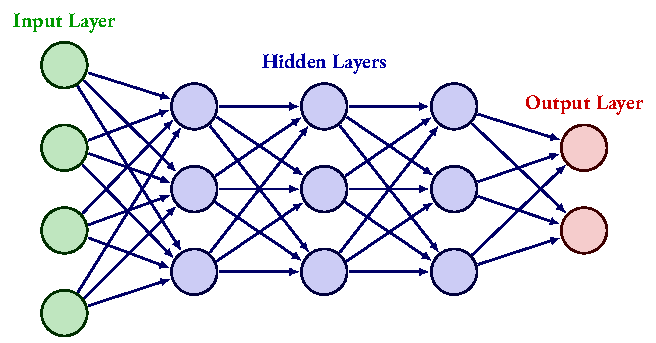
\includegraphics[scale=1.4]{tikz/chapter1 - Feedforward Neural Network.pdf}
    \caption{Example of a Feedforward Neural Network}
\end{figure}

A feedforward neural network can be thought of as a sequence of features, each of which represents a layer of the network. This structure is based on the composition of these functions to form an overall representation of the input data. Formally, we can represent a feedforward network as a composition of several functions:
$$ f(\mathbf{x}) = f^{(i)}(f^{(i-1)}(\dots f^{(2)}(f^{(1)}(\mathbf{x})) \dots )) $$  
Where \( f^{(1)} \) is the first layer (or input layer), \( f^{(i)} \) represents the output of the \(i\)-th layer, and so on. The depth of the network is defined by the number of layers, that is, the number of functions \( f^{(i)} \) involved.

In evaluating the functions of a feedforward network, which is acyclic graph, the flow of information proceeds in a single direction, from input to output. This flow passes through intermediate computations in the various layers of the network. 

In the initial layer, also called \textbf{\color{green!60!black}{Input Layer}}, each node corresponds to an input feature or variable, indeed there are no calculations or transformations applied to the data here.

Instead, neurons in the \textbf{\color{mybluee}{Hidden Layers}} perform nonlinear computations on the input data through the application of weights and activation functions.
The number of hidden layers and the number of neurons in each layer may vary depending on the architecture of the network and the complexity of the problem.
The main function of the hidden layers is to capture and represent complex and abstract features of the input data.

Finally in the \textbf{\color{red!80!black}{Output Layer}} we obtain the desired output.
The number of nodes in this layer depends on the nature of the problem, for example, in a binary classification problem there will be only one node, while in a multiclass classification problem there will be one node for each class.
Also the type of activation function used in the output layer depends on the type of problem the network is addressing! For example, for binary classification problems, the sigmoid activation function can be used, while for multiclass we use the softmax.

\subsection{Overcoming the limitations of linear models}

Linear models have long been used for their simplicity and convex optimization, but they have significant limitations in their ability to capture complex interactions between input variables. This limitation is particularly evident when dealing with complex problems such as nonlinear classification.

In the context of linear models, such as support vector machines, the choice of function \( \phi \) (\textbf{Nonlinear mapping of input data in feature space}) is crucial to satisfactory performance. However, there are limitations in engineering this function, which can make it difficult to capture complex information in the data. Below, we review three common options for addressing these challenges:
\begin{enumerate}
    \item \textbf{Use of generic \( \phi \)}: A first option is to use a generic \( \phi \) function. For example, in kernel machines with RBF (Radial Basis Function) kernels, \( \phi \) has implicit infinite dimensionality. This provides sufficient capacity to fit the training data. However, this approach may suffer from poor generalization for highly variable objective functions.
    \item \textbf{Engineer \( \phi \)}: Here, efforts are devoted to manually engineering a function that can capture the relevant information in the input data. However, this approach may be limited by the complexity of the data and the difficulty in correctly identifying key relationships.
    \item \textbf{Learning \( \phi \) from the data}: Finally, an option is to learn the \( \phi \) function directly from the data. This approach renounces convexity but offers significant advantages by combining the strengths of the first two options. \( \phi \) can be modeled very generically, and engineering can focus on designing neural network architectures capable of learning complex and informative representations from input data.
\end{enumerate}

Thanks to Feedforward Neural Networks we can overcome the limitations of traditional linear models because they are able to learn complex, nonlinear functions from data, thus overcoming the inherent limitations of linear models in capturing complex relationships between input variables.

The training of a neural network shares many similarities with that of other machine learning models. However, it has unique features that deserve to be explored. While it is essential to provide only the output of the final layers during training, the hidden layers do not require specific analysis during this phase, which contributes to the complexity and overall effectiveness of the network.

The main difference from linear models lies in the loss functions. While in linear models the loss is convex and guarantee convergence, in neural networks it become nonconvex, leading to greater complexity and not guaranteeing convergence to a global optimum.

Train a neural network means optimize the parameters' values $\mathbf{W}$ (wheights) in order to achieve $f(X,\mathbf{W})$ as close as the target unknown function $f(X)$. So, it is essential to apply gradient descent, an iterative approach to minimizing the cost function, and it is crucial to specify an appropriate \textbf{cost function} that accurately represents the error between the predicted output and the desired output. In addition, modeling choices may vary, including the selection of \textbf{output representation}, \textbf{activation functions}, and \textbf{network architecture} (e.g., number of layers), significantly affecting network performance.

Beyond that, there are other aspects of modeling that can be adapted to improve network performance, such as the choice of \textbf{optimizer} and the use of \textbf{regularization} techniques to avoid overfitting and improve generalization. 

To summarize, in a Neural Network we need to specify the following elements: cost function, output representation, activation function, architecture, optimizer, regularization.

\section{Cost Functions}

Cost (or Loss) functions play a key role in the training of deep learning models. They measure the \textbf{discrepancy between model predictions and actual target values} during the training process. An accurate choice of loss function is essential for optimal model performance.

For \textbf{Classification} problems, two commonly used loss functions are Categorical Cross-Entropy and Binary Cross-Entropy. These functions are designed to work with class probabilities and are particularly well suited for models that produce probability distributions.

{\Large
% $$
\begin{equation*}
\text{\textbf{Categorical Cross-Entropy}} = -\sum_{i=1}^{N} \tikzmarkk{Y}\textcolor{myred}{y_i} \log(\tikzmarkk{YC}\textcolor{mybluee}{\hat{y}_i})
\end{equation*}
\begin{tikzpicture}[overlay,remember picture]
    \node (Ye) [below of = Y, node distance = 3 em, anchor=west] {\footnotesize \textsf{\textcolor{myred}{true probability of class $i$}}};
    \draw[<-, in=180, out=-90] (Y.south)++(.25em,-1ex) to (Ye.west);

    \node (YCe) [below of = YC, node distance = 2 em, anchor=west] {\footnotesize \textsf{\textcolor{mybluee}{predicted probability of class $i$}}};
    \draw[<-, in=180, out=-90] (YC.south)++(.25em,-1ex) to (YCe.west);
\end{tikzpicture}
}

{\Large
% $$
\begin{equation*}
\text{\textbf{Binary Cross-Entropy}} = -\left(\tikzmarkk{Y}\textcolor{myred}{y}\log(\tikzmarkk{YC}\textcolor{mybluee}{\hat{y}}) + (1 - y) \log(1 - \hat{y})\right)
\end{equation*}
% $$
\begin{tikzpicture}[overlay,remember picture]
    \node (Ye) [below of = Y, node distance = 3 em, anchor=west] {\footnotesize \textsf{\textcolor{myred}{true label (0 or 1)}}};
    \draw[<-, in=180, out=-90] (Y.south)++(.25em,-1ex) to (Ye.west);

    \node (YCe) [below of = YC, node distance = 2 em, anchor=west] {\footnotesize \textsf{\textcolor{mybluee}{predicted probability of class 1}}};
    \draw[<-, in=180, out=-90] (YC.south)++(.25em,-1ex) to (YCe.west);
\end{tikzpicture}
}
\vspace{1cm}

In the case of \textbf{Regression}, different loss functions are used, including:

{\Large
% $$
\begin{equation*}
\text{\textbf{Mean Squared Error}} = \frac{1}{N} \sum_{i=1}^{N} (\tikzmarkk{Y}\textcolor{myred}{y_i} - \tikzmarkk{YC}\textcolor{mybluee}{\hat{y}_i})^2
\end{equation*}
% $$
\begin{tikzpicture}[overlay,remember picture]
    \node (Ye) [below of = Y, node distance = 3 em, anchor=west] {\footnotesize \textsf{\textcolor{myred}{actual (or true) target value for the example \( i \)}}};
    \draw[<-, in=180, out=-90] (Y.south)++(.25em,-1ex) to (Ye.west);

    \node (YCe) [below of = YC, node distance = 2 em, anchor=west] {\footnotesize \textsf{\textcolor{mybluee}{model prediction for the example \( i \)}}};
    \draw[<-, in=180, out=-90] (YC.south)++(.25em,-1ex) to (YCe.west);
\end{tikzpicture}
}
\vspace{1cm}

Mean Squared Error (MSE) calculates the mean squares of the differences between model predictions and actual values. It is commonly used and strongly penalizes significant errors. However, it is sensitive to outliers. 

% \newpage

{\Large
% $$
\begin{equation*}
\text{\textbf{Mean Absolute Error}} = \frac{1}{N} \sum_{i=1}^{N} |\tikzmarkk{Y}\textcolor{myred}{y_i} - \tikzmarkk{YC}\textcolor{mybluee}{\hat{y}_i}|
\end{equation*}
% $$
\begin{tikzpicture}[overlay,remember picture]
    \node (Ye) [below of = Y, node distance = 3 em, anchor=west] {\footnotesize \textsf{\textcolor{myred}{actual (or true) target value for the example \( i \)}}};
    \draw[<-, in=180, out=-90] (Y.south)++(.25em,-1ex) to (Ye.west);

    \node (YCe) [below of = YC, node distance = 2 em, anchor=west] {\footnotesize \textsf{\textcolor{mybluee}{model prediction for the example \( i \)}}};
    \draw[<-, in=180, out=-90] (YC.south)++(.25em,-1ex) to (YCe.west);
\end{tikzpicture}
}
\vspace{1cm}

Mean Absolute Error (MAE), or only Absolute Error (AE), calculates the mean of the absolute differences between predictions and actual values. It is less sensitive to outliers than MSE, but its derivative is undefined in zero.

{\Large
% $$
\begin{equation*}
\text{\textbf{Huber Loss}} = \frac{1}{N} \sum_{i=1}^{N} \left\{
\begin{array}{ll}
    \frac{1}{2} (y_i - \hat{y}_i)^2 & \text{se } |y_i - \hat{y}_i| \leq \textcolor{mygreen}{\delta} \\
    \tikzmarkk{D}\textcolor{mygreen}{\delta} (|y_i - \hat{y}_i| - \frac{1}{2} \textcolor{mygreen}{\delta}) & \text{otherwise}
\end{array}
\right.
\end{equation*}
% $$
\begin{tikzpicture}[overlay,remember picture]
    \node (De) [below of = D, node distance = 2.5 em, anchor=west]     {\parbox{\widthof{hyperparameter controlling the transition between}}{
    \ \\
    \footnotesize \textsf{\textcolor{mygreen}{hyperparameter controlling the transition between}} \\ 
    \footnotesize \textsf{\textcolor{mygreen}{the quadratic and linear regions of the loss function}}}};
    \draw[<-, in=180, out=-90] (D.south)++(.25em,-.5ex) to (De.west);
\end{tikzpicture}
}
\vspace{1cm}

Huber Loss combines the best features of MSE and MAE. For small errors, it behaves similar to MSE, while for larger errors, it behaves like AE. This avoids problems such as overfitting and steep slope of the MSE curve.

\textit{\textbf{Please Note}}: There are numerous other loss functions besides those mentioned above, which can be used depending on the specific problem to be addressed and the characteristics of the data. The choice of loss function depends on the goal of model training, the nature of the data, and the needs of the application. For example, in special contexts such as outlier detection or handling noisy data, specialized loss functions might be preferred. Moreover, as deep learning research advances, new loss functions are constantly being developed and existing ones adapted to meet emerging challenges in different application scenarios. 

\textit{\textbf{Also}}: The choice of the cost function is not independent of the choice of the output unit, because choosing one specific output unit over another can be convenient for the cost function we want to use (e.g., sigmoid and binary cross-entropy).

\section{Unit Types}

\subsection{Linear Units}

Linear Units play a key role in the intermediate and output layers of neural networks. These units apply a \textbf{linear transformation to the inputs} by combining the weights associated with the inputs with the input values themselves. The output produced by Linear Units is a linear combination of the inputs. 

The formula for calculating the output of Linear Units is:
$$
\hat{y} = W^T h + b
$$
Where \( \hat{y} \) represents the predicted output, \( W \) are the weights associated with the inputs, \( h \) represents the features from the previous layer, and \( b \) is the bias term.

\subsection{Softmax Units}

Softmax Units are commonly used in the output layers of neural networks, especially in cases of Multiclass Classification (with Cross-Entropy Loss). These units transform the un-normalized scores from the last linear layer into a \textbf{normalized probability distribution}, allowing the model to assign a probability to each membership class for a given input.

The softmax formula used to calculate the probabilities is as follows:
$$
\text{Softmax}(z_i) = \frac{e^{z_i}}{\sum_{j} e^{z_j}}
$$
Where \( z_i \) represents the non-normalized score associated with the class \( i \), and \( \sum_{j} e^{z_j} \) is the sum of all the exponents of the non-normalized scores.

Log Softmax is a variant of the Softmax function that is used to \textbf{improve numerical stability} when computing probabilities. The formula for calculating the Log Softmax is as follows:
$$
\text{log Softmax}(z_i) = z_i - \log\left(\sum_{j} e^{z_j}\right)
$$

Here are some advantages:
\begin{itemize}
    \item \textbf{The term \( z_i \) never saturates}: This means that the scale of values \( z_i \) is not compressed or restricted in any way. This is beneficial because it allows the model to continue to learn from more relevant information without limitations imposed by value saturation.
    
    \item \textbf{Maximizing the log-likelihood encourages \( z_i \) to be increased, while encouraging all other \( z \) to be decreased}: When we maximize the log-likelihood, we are trying to make the model's prediction as close to reality as possible. Thus, we encourage \( z_i \) to increase, since it represents the probability associated with the correct class. At the same time, we encourage the other \( z \) to decrease to reduce the probability associated with the wrong classes.
    
    \item \textbf{The log-likelihood cost function heavily penalizes the most active incorrect prediction}: The log-likelihood cost function significantly penalizes the most active incorrect prediction. This means that if the model is very sure of an incorrect prediction (for example, it has a very high probability for an incorrect class), the cost function will increase significantly, encouraging the model to correct that error.
\end{itemize}

This analysis prompts us to consider a fundamental question: \textit{How can we select the activation function $h$ most suitable for our neural network?}

In the next section, we try to answer this crucial question! 
We have decided to be quite descriptive, as we believe that more details about these functions can facilitate a deeper understanding.

\section{Activation Functions}

\subsection{Sigmoid}

\begin{table}[h]
\begin{tabularx}{\linewidth}{>{\parskip1ex}X@{\kern4\tabcolsep}>{\parskip1ex}X}
\toprule
\hfil\bfseries \color{mybluee}{Pros}
&
\hfil\bfseries \color{mybluee}{Cons}
\\\cmidrule(r{3\tabcolsep}){1-1}\cmidrule(l{-\tabcolsep}){2-2}

%% PROS
The sigmoid function offers a valuable advantage because it acts as a type of \textbf{\textcolor{mybluee}{squashing non-linearity}} that "squeezes" outputs within the range of [$0$, $1$]. This feature is particularly advantageous in scenarios such as binary classification tasks, where the model must generate outputs that can be interpreted as probabilities.

Moreover, the sigmoid function has a property of \textbf{\textcolor{mybluee}{differentiability and smoothness}} over its entire domain. This property facilitates seamless integration with gradient-based optimization techniques, ensuring stable convergence during the training process.
&

%% CONS
However, it \textbf{\textcolor{mybluee}{tends to saturate}} in most of its domain. This saturation phenomenon causes the gradient to tend toward zero, posing challenges during the learning phase. Consequently, this saturation can obstruct the effective propagation of gradients through the network during back-propagation.

In addition, the sigmoid function shows strong sensitivity mainly when the input is near zero. In contrast, its \textbf{\textcolor{mybluee}{sensitivity decreases}} for both large and small input values. This characteristic negatively affects the model's ability to learn from datasets that have a wide range of input values.
\\\bottomrule
\end{tabularx}
\caption{Benefits and Limitations of Sigmoid Activation}
\end{table}

\vspace{1cm}
\begin{figure}[!htbp]
    \centering
    \includegraphics[scale=2]{tikz/chapter1 - Sigmoid.pdf}
    \caption{Sigmoid Activation Function Plot}
\end{figure}

\newpage
\subsection{Hyperbolic Tangent}

\begin{table}[h]
\begin{tabularx}{\linewidth}{>{\parskip1ex}X@{\kern4\tabcolsep}>{\parskip1ex}X}
\toprule
\hfil\bfseries \color{myred}{Pros}
&
\hfil\bfseries \color{myred}{Cons}
\\\cmidrule(r{3\tabcolsep}){1-1}\cmidrule(l{-\tabcolsep}){2-2}

%% PROS
First, it is \textbf{\textcolor{myred}{differentiable and continuous}}, ensuring compatibility with gradient-based optimization techniques. 

In addition, the hyperbolic tangent function is \textbf{\textcolor{myred}{similar to sigmoid}}, but provides a more favorable output range. By squashing the outputs in the interval [$-1$, $1$], it ensures that the outputs are centered in zero. This feature can improve the model's ability to learn and adapt to data distributions, especially in scenarios where centered data is advantageous.
&

%% CONS
However, the hyperbolic tangent function also has limitations. Like the sigmoid, it tends to \textbf{\textcolor{myred}{saturate}} throughout much of its domain. This saturation phenomenon can hinder effective gradient propagation during back-propagation, impeding the learning process and potentially leading to slower convergence.
\\\bottomrule
\end{tabularx}
\caption{Benefits and Limitations of Hyperbolic Tangent Activation}
\end{table}

\vspace{1cm}
\begin{figure}[!htbp]
    \centering
    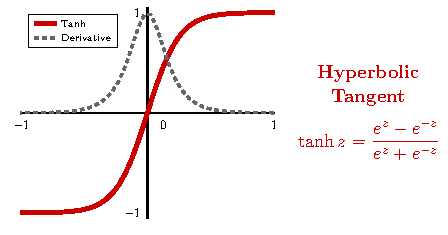
\includegraphics[scale=2]{tikz/chapter1 - Hyperbolic Tangent.pdf}
    \caption{Hyperbolic Tangent Activation Function Plot}
\end{figure}

\newpage
\subsection{Rectified Linear Unit (ReLU)}
\begin{table}[h]
\begin{tabularx}{\linewidth}{>{\parskip1ex}X@{\kern4\tabcolsep}>{\parskip1ex}X}
\toprule
\hfil\bfseries \color{mygreen!80!black}{Pros}
&
\hfil\bfseries \color{mygreen!80!black}{Cons}
\\\cmidrule(r{3\tabcolsep}){1-1}\cmidrule(l{-\tabcolsep}){2-2}

%% PROS
The ReLU function has several advantages. First, it provides \textbf{\textcolor{mygreen!80!black}{wide and consistent gradients}} when it is active. This means that the ReLU function does not saturate when it is active, which greatly accelerates the convergence of gradient-based optimization.
In addition, the \textbf{\textcolor{mygreen!80!black}{non-positive limitation}} accelerates the convergence of gradient descent, allowing for faster learning.
The ReLU function may have a limitation in its \textbf{\textcolor{mygreen!80!black}{differentiability}}. However, in practice, this is not necessarily a problem since the one-sided derivative is returned when \( z = 0 \). Moreover, gradient-based optimization is subject to numerical errors anyway, so this differentiability limitation is often overlooked.
A good practice is to \textbf{\textcolor{mygreen!80!black}{initialize bias}} with small positive values. This ensures that units are initially active for most inputs and that derivatives can propagate through.
&

%% CONS
However, the ReLU function also has some disadvantages. First of all, its outputs are not \textbf{\textcolor{mygreen!80!black}{centered on zero}}, which could cause problems in some machine learning contexts.
In addition, ReLU neurons may suffer from a phenomenon called \textbf{\textcolor{mygreen!80!black}{"dying ReLU"}}. This occurs when most of the inputs to ReLU neurons are in the negative range. When this occurs, the ReLU neurons return an output of $0$ and the gradients do not flow during back-propagation, preventing the weights from updating. However, this problem does not always occur and can be mitigated by properly adjusting the learning rate or using Stochastic Gradient Descent (SDG).
The ReLU function can also be sensitive to the \textbf{\textcolor{mygreen!80!black}{large learning rate}}. If the learning rate is too high, the new weights are likely to end up in the highly negative range, negatively affecting the convergence of the model.
\\\bottomrule
\end{tabularx}
\caption{Benefits and Limitations of ReLU Activation}
\end{table}

\vspace{1cm}
\begin{figure}[!htbp]
    \centering
    \includegraphics[scale=2]{tikz/chapter1 - ReLU.pdf}
    \caption{ReLU Activation Function Plot}
\end{figure}


\subsection{Generalized Rectified Linear Units}

The \textbf{generalized rectified linear units} were introduced to address some limitations of the ReLU function. The main objective is to obtain a non-zero slope when \( z_i < 0 \). The generalized form of the ReLU is defined as follows:
$$ h(z, \alpha_i) = \max(0, z_i) + \alpha_i \min(0, z_i) $$
However, generalized rectified linear units are not universally better than ReLU and may lead to other problems, such as additional computational complexity. Some of the improvements that have been made include:
\begin{itemize}     
    \item \textbf{Leaky ReLU}: This variation solves the problem of neuron death by setting \( a_i \) to a small value, such as $0.01$, to maintain a gradient flow even when the input is negative.
    \item \textbf{Parametric ReLU}: This variant allows the parameter \( a_i \) to be learned, allowing the network to adapt the gradient of the activation function based on the data.
    \item \textbf{ReLU Randomized}: This variant samples the parameter \( a_i \) from a fixed interval during training and keeps it constant during testing, introducing randomness into the model.
\end{itemize}

In addition, other activation functions have been proposed as alternatives to ReLU, including:
\begin{itemize}     
    \item \textbf{Exponential Linear Units (ELU)}: This activation function retains all the advantages of ReLU but avoids the problem of neuron death. However, it requires exponentiation during computation, slightly increasing the computational complexity.
    \item \textbf{Swish}: This function is a smooth, non-monotonic function that has been shown to perform better than ReLU on deeper models, improving performance on datasets such as ImageNet.
    \item \textbf{Linear Units with Gaussian Error (GELU)}: This activation function has been used in state-of-the-art algorithms such as GPT-3 and BERT. It combines the non-monotonic aspect (that helps for the gradient of the function),  regularization techniques such as dropout and zone-out, and ReLU benefits to achieve a smoother version of ReLU. 
\end{itemize}

% These improvements and generalizations of activation functions have helped make neural networks more efficient and adaptable to a wide range of machine learning problems. Below, we show graphs of the Leaky ReLU and ELU activation functions for a better understanding of their properties.

\begin{figure}[!htbp]
    \centering
    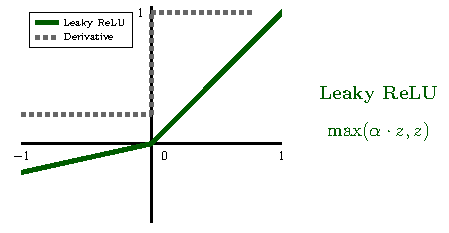
\includegraphics[scale=2]{tikz/chapter1 - Leaky ReLU.pdf}
    \caption{Leaky ReLU Activation Function Plot}
\end{figure}

\begin{figure}[!htbp]
    \centering
    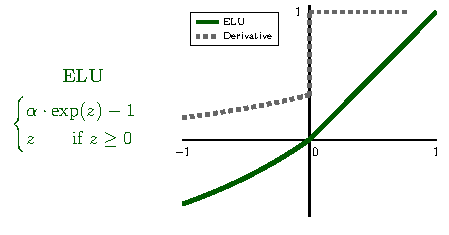
\includegraphics[scale=2]{tikz/chapter1 - ELU.pdf}
    \caption{ELU Activation Function Plot}
\end{figure}

\section{Architecture design}
\textit{How do we decide depth and width?} Choosing the depth and width of a neural network depends on several factors, including the complexity of the problem to be solved, the availability of training data, and the computational resources available. In principle, how many hidden layer units are sufficient? Theory offers us some answers.

\begin{remark}
Cybenko's Theorem (1989), also known as the universal approximation theorem, states that \textbf{a two-layer neural network with linear output can approximate any continuous function} over a compact domain with arbitrary precision, provided there are enough hidden units. This theorem has important implications for the design of neural architectures.
\end{remark}

\textbf{Implications}: Regardless of the function we are trying to learn, we know that a large multilayer neural network can represent this function. However, there is no guarantee that our training algorithm will be able to learn that function, due to optimization or data overlap issues. Also, the theorem gives no indication of how large the network will be.

\textit{So is depth or width more important?} There are trade-offs between depth and width of neural networks. For example, deeper networks generally generalize better: imagine a neural network as a set of tools to solve a problem. The more tools you have, the more complex problems you can solve. Then, by adding more "layers" to the network (making it deeper), we could give the network the ability to tackle more difficult problems or capture finer details in the data. In addition, architecture design has a significant impact on performance, for example between convolutional and feedforward neural networks.

\newpage
\chapter{Backpropagation} 
\section{The Gradient Descent Algorithm}

\vspace{-0.4cm}
To train neural networks effectively, we employ the (Stochastic) \textbf{Gradient Descent algorithm} in combination with \textbf{Backpropagation}. Backpropagation, a method for computing gradients, is crucial for updating the parameters of the neural network during training. We will delve into it shortly, but first, let's explore Gradient Descent and its significance.
\vspace{-0.4cm}

\subsection{Understanding the Gradient}

Gradient Descent is a fundamental optimization algorithm used to minimize the loss function of a neural network by iteratively adjusting its parameters. The goal is to find the optimal set of parameters that result in the lowest possible loss. The algorithm works by iteratively moving in the \textbf{direction of the steepest descent of the loss function} with respect to the parameters. This direction is determined by the \textbf{negative gradient} of the loss function, which is why we will utilize the negative sign in the algorithm.

Mathematically, the update rule for the parameters \( w \) in Gradient Descent can be expressed as:
$$
\Delta_w L = \left[ \frac{\partial L}{\partial w_1}, \frac{\partial L}{\partial w_2}, \ldots , \frac{\partial L}{\partial w_N}\right]
$$
where \( \Delta_w L \) represents the change in the loss function \( L \) with respect to the parameters \( w \), and \( \frac{\partial L}{\partial w_i} \) denotes the partial derivative of the loss function with respect to the \( i \)-th parameter \( w_i \).

Below we show a figure illustrating the partial derivatives of a function. The figure is represented in two ways: in a 3D graph and in the two-dimensional projection of the same graph (top view). The surface of the graph represents the function, where the lowest point is colored blue and the highest point is colored red. The black arrows extending from the surface indicate the direction and intensity of the gradient change of the function at each point in space. This visualization is crucial for understanding how Gradient Descent finds the fastest direction to reduce loss and update model weights during neural network training.

\begin{figure}[!htbp]
    \centering
    \includegraphics[scale=2]{tikz/chapter2 - Partial Derivatives.pdf}
    \caption{Visualization of Partial Derivatives in Two Distinct Ways}
\end{figure}

Having understood partial derivatives and the role of the gradient in the optimization process, let's now look at a visual representation of how the Gradient Descent algorithm works. In the image below, we see a three-dimensional surface representing the loss function. As before, the lowest point of the surface is colored blue and represents the minimum of the loss function. The black arrows extending from the surface indicate the \textbf{path} that Gradient Descent follows \textbf{to reach the minimum}. Each arrow represents the direction and intensity of the change in the loss function at a given point in space.

\begin{figure}[!htbp]
    \centering
    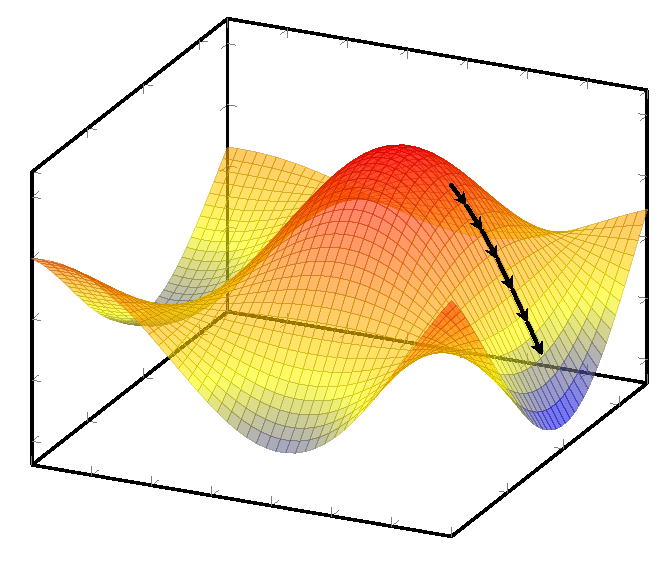
\includegraphics[scale=0.75]{tikz/chapter2 - Gradient Descent.pdf}
    \caption{Visual Representation of the Gradient Descent Algorithm}
\end{figure}

The algorithm proceeds by iteratively updating the parameters according to the gradient direction \textbf{until convergence is reached or a predefined number of iterations is completed}. By following this process, Gradient Descent effectively navigates the parameter space to find the optimal configuration that minimizes the loss function.


\subsection{The Problem of Local Minima}

In neural networks, the optimization problem is non-convex, leading to the existence of \textbf{local minima}. However, practitioners have found that these local minima are often still effective solutions. Thus, local minima are not typically a significant concern in neural network training. Below, we show an example illustrating the local minima problem for a better insight.

\begin{figure}[!htbp]
    \centering
    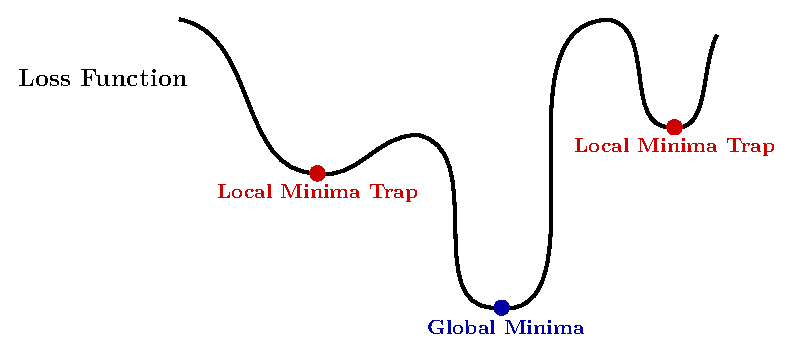
\includegraphics[scale=0.9]{tikz/chapter2 - Local Minima.pdf}
    \caption{Local and Global Minima}
\end{figure}

\subsection{The Problem of Sad\partial Le Points}

Another optimization challenge arises from sad\partial Le points, where some directions curve upwards and others downwards. At a sad\partial Le point, the \textbf{gradient is zero}, even if the point is not a minimum. Sad\partial Le points are common in high-dimensional spaces. However, they only become problematic if the optimization algorithm becomes stuck exactly at the sad\partial Le point.

\begin{figure}[!htbp]
    \centering
    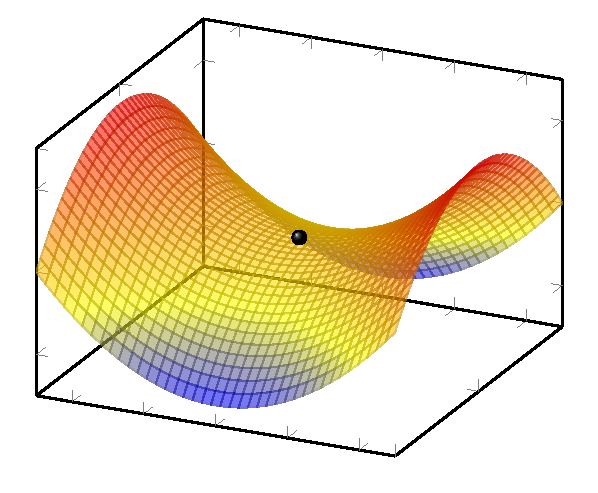
\includegraphics[scale=0.88]{tikz/chapter2 - Saddle Point.pdf}
    \caption{Saddle Le Point Illustration}
\end{figure}

In the figure, there is a saddle point depicted within the neural network optimization scenario, represented by the black dot. 

\section{Backpropagation Algorithm}

\subsection{Backpropagation Fundamentals}
How do we learn the weights of a neural network? Let us examine some ideas that have guided the development of learning algorithms in the context of neural networks.

The initial idea was to \textbf{randomly perturb one weight at a time}, evaluating whether that change improved model performance and saving the change. This approach, although similar to an evolutionary process, proved to be very inefficient, requiring numerous passes over the training data for each change in the weights and presenting difficulties in the last stage of learning.

Another idea involved \textbf{perturbing all the weights simultaneously} and correlating performance improvement with changes in the weights. However, this method proved equally inefficient and extremely difficult to implement.

Subsequently, a more efficient idea was proposed: to \textbf{perturb only the activations}, which are fewer in number than the weights. Although this approach is an improvement over the previous ones, it is still inefficient.

\textit{Therefore, how can we achieve more efficient learning?} This is where backpropagation comes in.

\begin{remark}
Backpropagation is a widely used learning algorithm in neural networks, which consists of three main steps:

\begin{enumerate}
    \item \textbf{Forward Propagation}: summation of inputs, production of activations and propagation of output through the network.

    \item \textbf{Error Estimation}: comparison of labels with predictions obtained from the network.

    \item \textbf{Backpropagation} of the error signal and using this signal to update the weights by computing gradients.
\end{enumerate}
\end{remark}

Starting from the training data, we do not directly know the optimal behavior of the hidden units within the neural network. However, using backpropagation, we can calculate how quickly the overall error of the network changes when we change the activity of these hidden units.

Using the derivatives of the error with respect to the hidden activities, we are able to understand \textbf{how each hidden unit affects the overall error of the network}. This allows us to gain a clear view of the separate effects that each hidden unit has on the error and how these effects are combined to determine the optimal direction to update the network weights.

Once we have calculated the derivatives of the error with respect to the hidden activities, we gain valuable information to update the weights associated with each connection in the network. This allows us to adjust the weights in a way that minimizes the overall error in the network, moving us closer and closer to the optimal solution for the learning problem.

\section{Exploring Backpropagation: Step by Step}

In this section, we will explore backpropagation of the error through a neural network in detail, starting with the output layer and proceeding to the input layer. We begin with a neural network composed of \textbf{one neuron per layer}.

\begin{minipage}{0.45\textwidth}
\includegraphics[width=\textwidth]{tikz/chapter2 - Chain Rule One Layer.pdf}
\captionof{figure}{Conceptualisation of Calculations}
\end{minipage}
\begin{minipage}{0.55\textwidth}
After performing the forward step, we will get an output from the last activation \( a^{(l)} \), which will allow us to calculate the loss \( \textcolor{myred}{L} \) using the desired output \( y \). The latter activation \( a^{(l)} \) is calculated using three elements: a weight \( \textcolor{myblue}{w^{(l)}} \), a bias \( \textcolor{myorange}{b^{(l)}} \), and the activation of the preceding neuron \( a^{(l-1)} \). The resulting equations are as follows:

$$ \textcolor{mygreen}{z^{(l)}} = \textcolor{myblue}{w^{(l)}} a^{(l-1)} + \textcolor{myorange}{b^{(l)}} $$
$$ a^{(l)} = \sigma(\textcolor{mygreen}{z^{(l)}}) $$
Where \textcolor{mygreen}{$z^{(l)}$} is the input of a non-linear function $\sigma$, such as a sigmoid or a ReLU. \\

A way you might conceptualize this is that the weight \( \textcolor{myblue}{w^{(l)}} \), the prior activation \( a^{(l-1)} \), and the bias \( \textcolor{myorange}{b^{(l)}} \) together \textbf{\textcolor{myyellow!85!black}{allow us to calculate}} \( \textcolor{mygreen}{z^{(l)}} \), which in turn \textbf{\textcolor{myyellow!85!black}{allow us to calculate}} \( a^{(l)} \), which together with the desired output \( y \) \textbf{\textcolor{myyellow!85!black}{allows us to calculate the loss}} \( \textcolor{myred}{L} \). This concept is illustrated in the diagram on the left.
\end{minipage}

Our initial goal during the backward step is to understand how sensitive the loss \( \textcolor{myred}{L} \) is to small changes in the weight \( \textcolor{myblue}{w^{(l)}} \), that is, calculate the derivative\( \frac{\textcolor{myred}{\partial L}}{\textcolor{myblue}{\partial w^{(l)}}} \). 
Conceptually, when you see this kind of formula, we need to think of it as saying to us "\textbf{how much does \( \textcolor{myred}{L} \) (numerator) change if we make a small change at \( \textcolor{myblue}{w^{(l)}} \) (denominator)?}"

When we calculate this derivative, we note that a small change in weight \( \textcolor{myblue}{w^{(l)}}\) \textbf{\textcolor{myyellow!85!black}{causes a change in}} \( \textcolor{mygreen}{z^{(l)}} \), which in turn \textbf{\textcolor{myyellow!85!black}{causes a change in}} \( a^{(l)} \), \textbf{\textcolor{myyellow!85!black}{directly affecting}} the loss \( \textcolor{myred}{L} \). And so this is where the chain of derivatives rule comes into play! 

As can be seen below we can now "chunk" the previous derivative:

\vspace{-0.8cm}
{\Large
% $$
\begin{equation*}
\hspace*{1cm}
\frac{\textcolor{myred}{\partial L}}{\textcolor{myblue}{\partial w^{(l)}}} = \frac{\textcolor{mygreen}{\partial z^{(l)}}}{\textcolor{myblue}{\partial \tikzmarkk{Z}w^{(l)}}}  
\frac{\partial a^{(l)}}{\textcolor{mygreen}{\partial \tikzmarkk{Y}z^{(l)}}} \frac{\textcolor{myred}{\partial L}}{\partial \tikzmarkk{YC}a^{(l)}}
\end{equation*}
% $$
\begin{tikzpicture}[overlay,remember picture]
    \node (Ze) [below of = Z, node distance = 4 em, anchor=west] {\footnotesize How much does a little variation to \( \textcolor{myblue}{w^{(l)}} \) changes \( \textcolor{mygreen}{z^{(l)}} \)?};
    \draw[<-, in=180, out=-90] (Z.south)++(.25em,-1ex) to (Ze.west);

    \node (Ye) [below of = Y, node distance = 3 em, anchor=west] {\footnotesize How much does a little variation to \( \textcolor{mygreen}{z^{(l)}} \) changes \( a^{(l)} \)?};
    \draw[<-, in=180, out=-90] (Y.south)++(.25em,-1ex) to (Ye.west);

    \node (YCe) [below of = YC, node distance = 2 em, anchor=west] {\footnotesize How much does a little variation to \( a^{(l)} \) changes \( \textcolor{myred}{L} \)?};
    \draw[<-, in=180, out=-90] (YC.south)++(.25em,-1ex) to (YCe.west);
\end{tikzpicture}
}
\vspace{1.8cm}

\textit{What about the bias term? Easy peasy!} We use the same method as for the weight term:

\vspace{-0.3cm}
$$\frac{\textcolor{myred}{\partial L}}{\textcolor{myorange}{\partial b^{(l)}}} = \frac{\textcolor{mygreen}{\partial z^{(l)}}}{\textcolor{myorange}{\partial b^{(l)}}}  \frac{\partial a^{(l)}}{\textcolor{mygreen}{\partial z^{(l)}}} \frac{\textcolor{myred}{\partial L}}{\partial a^{(l)}}$$

\textit{Now what? For the other layers?} Let's go back to our scheme for a moment and extend it:

\begin{figure}[htbp]
\centering
\includegraphics[width=\textwidth]{tikz/chapter2 - Chain Rule Multiple Layer.pdf}
\caption{Conceptualisation of Calculations (Extended)}
\end{figure}

All other weights and biases are in the earlier layers of the network, which means that their influence on cost is less direct. The way we han\partial Le them is to first consider how sensitive the cost is to the value of that activation in the penultimate layer, \( a^{(l-1)} \), and then consider how sensitive that value is to all the previous weights and biases.

The derivative of cost with respect to that activation looks a lot like what we have already seen:

\vspace{-0.5cm}
$$\frac{\textcolor{myred}{\partial L}}{\partial a^{(l-1)}} = \frac{\textcolor{mygreen}{\partial z^{(l)}}}{\partial a^{(l-1)}}  \frac{\partial a^{(l)}}{\textcolor{mygreen}{\partial z^{(l)}}} \frac{\textcolor{myred}{\partial L}}{\partial a^{(l)}}$$

The trick here is to remember that the activation in the previous layer is determined by its set of weights and biases. For example, there is a long chain of dependencies between the weight \( w^{(l-1)} \) and the cost \( \textcolor{myred}{L} \). The way this presents itself mathematically is that the partial derivative of the cost with respect to that weight appears as a long chain of partial derivatives for each intermediate step, see the image below to visualize the concept graphically.

\begin{minipage}{0.55\textwidth}

Here is how you can decompose the derivative:

\vspace{-0.3cm}
$$\frac{\textcolor{myred}{\partial L}}{\textcolor{myblue}{\partial w^{(l-1)}}} = 
\frac{\textcolor{mygreen}{\partial z^{(l-1)}}}{\textcolor{myblue}{\partial w^{(l-1)}}}  
\frac{\partial a^{(l-1)}}{\textcolor{mygreen}{\partial z^{(l-1)}}} 
\underbrace{
\frac{\textcolor{mygreen}{\partial z^{(l)}}}{\textcolor{myblue}{\partial w^{(l)}}}  
\frac{\partial a^{(l)}}{\textcolor{mygreen}{\partial z^{(l)}}} 
\frac{\textcolor{myred}{\partial L}}{\partial a^{(l)}}}_\textrm{\Large$\frac{\textcolor{myred}{\partial L}}{\textcolor{myblue}{\partial w^{(l)}}}$}$$
\vspace{-0.3cm}
\ \\
By following the dependencies through our tree and multiplying together a long series of partial derivatives, we now \textbf{can calculate the derivative of the cost with respect to any weight or bias of the entire network}. \textit{We are simply applying the same idea of the chain rule that we have always used!} \\

And since we can get any derivative, we can calculate the entire gradient vector:
\vspace{-0.1cm}
$$
\Delta_w L = \left[ \frac{\textcolor{myred}{\partial L}}{\textcolor{myblue}{\partial w^{(1)}}}, \frac{\textcolor{myred}{\partial L}}{\textcolor{myorange}{\partial b^{(1)}}}, \ldots , \frac{\textcolor{myred}{\partial L}}{\textcolor{myblue}{\partial w^{(l)}}}, \frac{\textcolor{myred}{\partial L}}{\textcolor{myorange}{\partial b^{(l)}}},\right] 
$$
\vspace{-0.3cm}
\ \\
The job is done! At least for this network, now we must add more neurons for each layer. \textit{I know, you are crying inside, but actually, not much changes when we give the layers more neurons: it's just a few more indexes to keep track of \emoji{smile}}.

\vspace{1cm}

\end{minipage}
\begin{minipage}{0.45\textwidth}
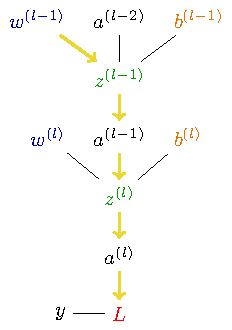
\includegraphics[width=\textwidth]{tikz/chapter2 - Chain Rule Multiple Layer Dependencies.pdf}
\captionof{figure}{Calculations with 3 Layers}
\end{minipage}

\begin{minipage}{0.4\textwidth}
\includegraphics[width=\textwidth]{tikz/chapter2 - Indexing.pdf}
\captionof{figure}{Neural Network Indexing}
\vspace{0.8cm}
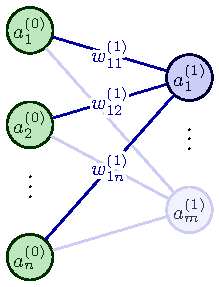
\includegraphics[width=\textwidth]{tikz/chapter2 - Indexing Example.pdf}
\captionof{figure}{Example of Indexing}
\end{minipage}
\begin{minipage}{0.05\textwidth}
\
\end{minipage}
\begin{minipage}{0.55\textwidth}
When dealing with neural networks with multiple neurons per layer, we have to change the notations a bit.\\

The activation of each neuron will be denoted with a subscript indicating its position within the layer. Thus, \textbf{the superscript of each neuron indicates which layer it is in, while the subscript indicates the specific neuron}.\\

The weights also need a refresh: additional indices are required to specify their location. In addition to the superscript representing the layer, \textbf{two subscripts indicate the edge weight connecting the neuron in layer $i$ to the neuron in layer $j$}.\\

\textit{I know, these "$ji$" indices, being backwards, might seem strange or unconventional at first, but they align with the way the weight matrix is usually indexed.}\\

On the left are two images: one formally represents how the nodes and edges of the network are represented, while the other provides an example with two dummy layers, named $0$ and $1$, with $n$ and $m$ nodes, respectively.
\end{minipage}

\newpage
The weighted sum \textcolor{mygreen}{$z_{j}^{(l)}$} then takes the following form:
$$
\textcolor{mygreen}{z_{j}^{(l)}} = \sum_{i} \textcolor{myblue}{w_{ji}^{(l)}} \cdot a_i^{(l-1)} + \textcolor{myorange}{b_{j}^{(l)}}
$$
The new equations turn out to be esentially the same with respect to the case of only one neuron per layer:

\vspace{-0.4cm}
$$
\frac{\textcolor{myred}{\partial L}}{\textcolor{myblue}{\partial w_{ji}^{(l)}}} = \frac{\textcolor{mygreen}{\partial z_{j}^{(l)}}}{\textcolor{myblue}{\partial w_{ji}^{(l)}}}  
\frac{\partial a_{j}^{(l)}}{\textcolor{mygreen}{\partial z_{j}^{(l)}}} \frac{\textcolor{myred}{\partial L}}{\partial a_{j}^{(l)}}
$$

Indeed, the expression of the derivative of the chain rule describing the sensitivity of cost with respect to a particular weight is the same as in the previous case. The only difference is that we now have multiple indices, $i$ and $j$, indicating which weight we are considering.

What changes, however, is the derivative of the cost with respect to one of the activations in the preceding layers, because \textbf{the preceding neurons influence the cost function through multiple pathways}.

To understand the sensitivity of the cost function with respect to a certain neuron, it is necessary to sum the influences along each of these different pathways. So, we \textbf{sum multiple expressions of different chain rules corresponding to each pathway of influence}.

\vspace{-0.5cm}
$$\frac{\textcolor{myred}{\partial L}}{\partial a_{i}^{(l-1)}} = \underbrace{\sum_{j}\frac{\textcolor{mygreen}{\partial z_{j}^{(l)}}}{\partial a_{i}^{(l-1)}}  \frac{\partial a_{j}^{(l)}}{\textcolor{mygreen}{\partial z_{j}^{(l)}}} \frac{\textcolor{myred}{\partial L}}{\partial a_{j}^{(l)}}}_\textrm{Sum over layer $l$}$$

This reasoning is carried out using traditional numerical values, but it is evident that in order to efficiently handle the weights and biases of the neural network, it is necessary to use the \textbf{matrix approach}, since it allows simultaneous operations to be performed on all the parameters of the network, greatly optimizing the computational process.


\newpage
\chapter{Optimization}
\vspace{-0.4cm}
In this chapter, we will immerse ourselves in optimization, exploring a wide range of gradient descent algorithms. We will start from the classic batch gradient descent to more advanced ones such as ADAM. But optimization does not stop there: we will also introduce a crucial element, data normalization, which contributes significantly to the effectiveness of our models. \textit{Ready to explore the nitty-gritty of these techniques? Let's dive in!}
\vspace{-0.4cm}

\section{Types of Gradient Descent}

\subsection{Batch Gradient Descent (BGD)}

The Batch Gradient Descent algorithm is one of the most widely used methods for parameter optimization in a neural network. Below we provide the algorithm.

\begin{algorithm}
\renewcommand\thealgorithm{}
\caption{\textbf{\textcolor{mygreen}{Batch Gradient Descent}}}
\begin{algorithmic}[1]
\REQUIRE{Learning Rate $\varepsilon$}
\REQUIRE{Initial Parameters $\mathbf{w}$}
\WHILE{Stopping Criteria not met}
    \STATE Compute gradient estimate on \textbf{\textcolor{myred}{$\mathbf{N}$ training examples}} $\{ (\mathbf{x}^{(1)}, y^{(1)}), ..., (\mathbf{x}^{(N)}, y^{(N)}) \}$
    \STATE $
    \mathbf{\hat{g}} \leftarrow \frac{1}{N}\nabla_{\mathbf{w}} \sum_{i=1}^{N} L(f(\mathbf{x}^{(i)},\mathbf{w}), y^{(i)})
    $
    \STATE Update parameters:
    $
    \textcolor{mybluee}{\mathbf{w} \leftarrow \mathbf{w} - \varepsilon \mathbf{\hat{g}}} 
    $
\ENDWHILE
\end{algorithmic}
\end{algorithm}

The distinguishing feature of Batch Gradient Descent is that it uses the \textbf{\textcolor{myred}{entire training dataset to calculate the gradient}} of the loss function. This means it requires \textbf{more computational resources and computation time} than other methods, but it can also lead to \textbf{more stable and accurate convergence}.
Therefore, Batch Gradient Descent remains one of the most widely used algorithms for training neural networks due to its conceptual simplicity and its effectiveness in learning model parameters. 

\subsection{Stochastic Gradient Descent (SGD)}

The Stochastic Gradient Descent algorithm, on the other hand, computes and applies parameter updates for each individual training example rather than using the entire training dataset. Below is the algorithm:

\begin{algorithm}
\renewcommand\thealgorithm{}
\caption{\textbf{\textcolor{mygreen}{Stochastic Gradient Descent}}}
\begin{algorithmic}[1]
\REQUIRE{Learning Rate $\varepsilon$}
\REQUIRE{Initial Parameters $\mathbf{w}$}
\WHILE{Stopping Criteria not met}
    \STATE Compute gradient estimate on \textbf{\textcolor{myred}{a random training example}} $(\mathbf{x}^{(i)}, y^{(i)})$
    \STATE 
    $
    \mathbf{\hat{g}} \leftarrow\nabla_{\mathbf{w}} L(f(\mathbf{x}^{(i)},\mathbf{w}), y^{(i)})
    $
    \STATE Update parameters:
    $
    \textcolor{mybluee}{\mathbf{w} \leftarrow \mathbf{w} - \varepsilon \mathbf{\hat{g}}}
    $
\ENDWHILE
\end{algorithmic}
\end{algorithm}

As we have mentioned, the distinguishing feature of Stochastic Gradient Descent is the use of \textbf{\textcolor{myred}{a single training example at a time}} to calculate the gradient and update the parameters. This method requires \textbf{less computational resources} than Batch Gradient Descent, but can be \textbf{more susceptible to fluctuations} during optimisation due to the variability introduced by individual training examples. However, SGD is often preferred when dealing with large data sets or when one wishes to frequently update parameters during training, as it can lead to faster convergence. 

\subsection{Mini-Batch Gradient Descent}
To mitigate the problem of noise or fluctuations associated with SGD, we can adopt the \textbf{\textcolor{mygreen}{Mini-Batch Gradient Descent}}. This variant of the algorithm applies parameter updates using a \textbf{\textcolor{myred}{fixed-sized subset of the training dataset}} at each iteration, known as a mini-batch, rather than using the entire dataset or a single training example. In this way, Mini-Batch Gradient Descent represents a compromise between the stability of Batch Gradient Descent and the computational efficiency of SGD.

The advantages of this approach are many. First of all, the computation time does not depend on the total size of the $N$ dataset, which makes it \textbf{suitable even for large datasets}. Furthermore, the method allows \textbf{parallel processing}, making it suitable for implementations on parallel hardware such as GPUs. However, this method has still a problem related to the optimization surface: along flat direction the gradient step is small so the algorithm achieves very slow progress, whereas if the surface is steep the may be jittery movements.  To solve this problem, \textit{momentum} have been developed.

\subsection{Stochastic Gradient Descent with Momentum}
Stochastic Gradient Descent with Momentum is a variant of the gradient descent algorithm that introduces a new variable, called \textit{velocity} (\(v\)), which represents an \textbf{exponentially decaying moving average} of negative gradients (in simple words, it tracks the progress history of the algorithm). The velocity accumulates the gradient over iterations, and it acts as a kind of "inertia" in the movement of the model parameters during learning, adding an acceleration component to the optimisation process.

\begin{algorithm}
\renewcommand\thealgorithm{}
\caption{\textbf{\textcolor{mygreen}{Stochastic Gradient Descent with Momentum}}}
\begin{algorithmic}[1]
\REQUIRE{Learning Rate $\varepsilon$}
\REQUIRE{Momentum Parameter $\alpha$}
\REQUIRE{Initial Parameters $\mathbf{w}$}
\REQUIRE{Initial Velocity $\mathbf{v}$}
\WHILE{Stopping Criteria not met}
    \STATE Compute gradient estimate on \textbf{\textcolor{myred}{a random training example}} $(\mathbf{x}^{(i)}, y^{(i)})$
    \STATE 
    $
    \mathbf{\hat{g}} \leftarrow\nabla_{\mathbf{w}} L(f(\mathbf{x}^{(i)},\mathbf{w}), y^{(i)})
    $
    \STATE Update the velocity:
    $\textcolor{mybluee}{\mathbf{v} \leftarrow \alpha \mathbf{v} - \varepsilon \mathbf{\hat{g}}}$
    \STATE Update the parameters:
    $\textcolor{mybluee}{\mathbf{w} \leftarrow \mathbf{w} + \mathbf{v}}$
\ENDWHILE
\end{algorithmic}
\end{algorithm}

The parameter \(\alpha\) controls the \textbf{\textcolor{mybluee}{contribution of the previous velocity}} in the current parameter update. If \(\alpha\) is greater than \(\varepsilon\), the current update is more influenced by the previous gradients, thus increasing \textbf{convergence stability} and helping the network to \textbf{avoid local minima}. 

Stochastic Gradient Descent with Momentum, while accelerating the process of reaching the minimum, can sometimes "overshoot" the desired target due to the inertia effect introduced by speed. However, it manages to reach the minimum much \textbf{faster than simple SGD}, making it an effective choice for optimising model parameters when training neural networks.


\begin{figure}[htbp]
\centering
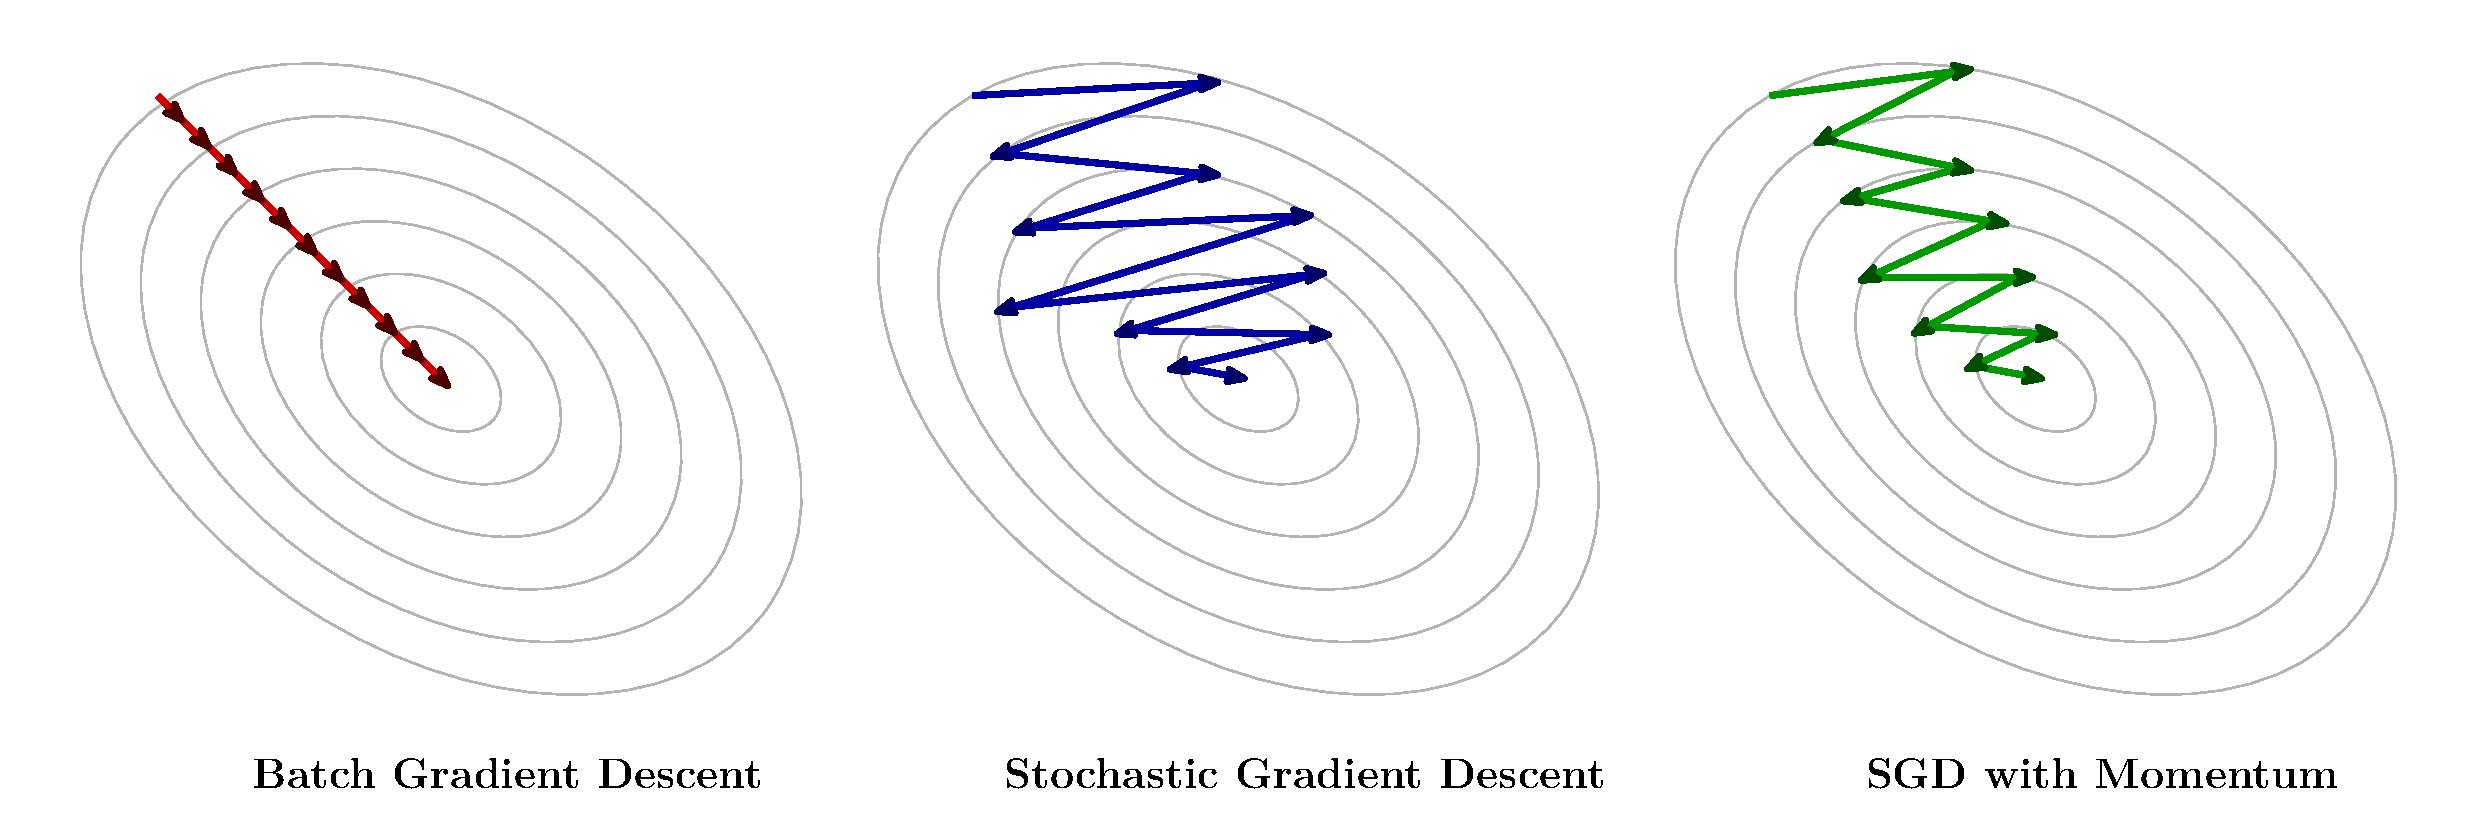
\includegraphics[width=\textwidth]{tikz/chapter3 - BGD vs SGD vs SGD with Momentum.pdf}
\caption{BGD vs SGD vs SGD with Momentum}
\end{figure}

\subsection{Stochastic Gradient Descent with Nesterov Momentum}

Stochastic Gradient Descent with Nesterov Momentum is a variant of the previous algorithm that adds a correction to the previous momentum before calculating the gradient. It works by firstly taking a step in the direction of the accumulated gradient (point 2 of the algorithm), and secondly calculating the gradient (point 4) and making the correction accordingly (point 5). (in simple momentum, we first compute the gradient and then make the correction) 

\begin{algorithm}
\renewcommand\thealgorithm{}
\caption{\textbf{\textcolor{mygreen}{Stochastic Gradient Descent with Nesterov Momentum}}}
\begin{algorithmic}[1]
\REQUIRE{Learning Rate $\varepsilon$}
\REQUIRE{Momentum Parameter $\alpha$}
\REQUIRE{Initial Parameters $\mathbf{w}$}
\REQUIRE{Initial Velocity $\mathbf{v}$}
\WHILE{Stopping Criteria not met}
\STATE Update parameters temporarily:
$\textcolor{mybluee}{\widetilde{\mathbf{w}} \leftarrow \mathbf{w} + \alpha \mathbf{v}}$
\STATE Compute gradient estimate on \textbf{\textcolor{myred}{a random training example}} $(\mathbf{x}^{(i)}, y^{(i)})$
\STATE $\mathbf{\hat{g}} \leftarrow \nabla_{\textcolor{mybluee}{\widetilde{\mathbf{w}}}} L(f(\mathbf{x}^{(i)},\textcolor{mybluee}{\widetilde{\mathbf{w}}}), y^{(i)})$
\STATE Update velocity:
$\textcolor{mybluee}{\mathbf{v} \leftarrow \alpha \mathbf{v} - \varepsilon \mathbf{\hat{g}}}$
\STATE Update parameters:
$\textcolor{mybluee}{\mathbf{w} \leftarrow \mathbf{w} + \mathbf{v}}$
\ENDWHILE
\end{algorithmic}
\end{algorithm}

The main difference between the Nesterov momentum and the standard momentum lies in \textbf{where the gradient is evaluated}. In the Nesterov momentum the gradient term is not calculated from the current position in parameter space, but rather from an intermediate position. This approach offers a significant advantage: while the gradient term always points in the optimal direction, \textbf{the momentum term may not align consistently}. Consequently, if the momentum goes in the wrong direction or overshoots the target, the gradient term can still "go back" and correct it \textbf{in the same update step}.

\newpage
\subsection{Adagrad (Adaptive Gradient Algorithm)}
The previous techniques that we have seen are based on the intuition of adjusting the learning rate while considering the history of past progress.

However, in many machine learning situations, we are faced with two distinct scenarios: a simpler one, in which all features are equally important, and a more difficult one, in which features have different levels of importance. However, up to this point, we have assigned the same learning rate to all features. \textit{Is this a valid idea?}

\begin{figure}[htbp]
\centering
\includegraphics[width=0.8\textwidth]{tikz/chapter3 - Features Importance.pdf}
\caption{Adaptive Learning Methods Intuition}
\end{figure}

Adagrad is an optimisation algorithm that \textbf{scales the model parameters by the square root of the sum of the squares of all historical gradient values}. This approach makes it possible to automatically adapt the learning rate for each parameter according to its update rate (in simple words, we take into account how much progress we have already done along each dimension and adjust the learning rate accordingly). 
\begin{algorithm}
\renewcommand\thealgorithm{}
\caption{\textbf{\textcolor{mygreen}{Adagrad}}}
\begin{algorithmic}[1]
\REQUIRE{Learning Rate $\varepsilon$}
\REQUIRE{Initial Parameters $\mathbf{w}$}
\REQUIRE{Small Constant $\delta$ to avoid division by zero}
\STATE Initialize sum of squared gradients vector: $\mathbf{r} \leftarrow 0$
\WHILE{Stopping Criteria not met}
\STATE Compute gradient estimate on \textbf{\textcolor{myred}{a random training example}} $(\mathbf{x}^{(i)}, y^{(i)})$
\STATE $\mathbf{\hat{g}} \leftarrow \nabla_{\mathbf{w}} L(f(\mathbf{x}^{(i)},\mathbf{w}), y^{(i)})$
\STATE Accumulate:
$\textcolor{mybluee}{\mathbf{r} \leftarrow \mathbf{r} + \mathbf{\hat{g}} \odot \mathbf{\hat{g}}}$
\STATE Update parameters:
$\textcolor{mybluee}{\mathbf{w} \leftarrow \mathbf{w} - \frac{\varepsilon}{\delta + \sqrt{\mathbf{r}}} \odot \mathbf{\hat{g}}}$ 
\ENDWHILE
\end{algorithmic}
\end{algorithm}

Where $\odot$ denotes element-wise multiplication.

Parameters that have large partial derivatives with respect to loss will see their learning rates reduced quickly, while those with smaller gradients will have higher learning rates, allowing for a \textbf{more stable convergence} of the model as not all direction of the optimization surface will have the same importance. 

\subsection{RMSProp (Root Mean Square Propagation)}

In many optimisation situations, Adagrad can excessively decrease the learning rate, making convergence difficult, especially in non-convex contexts. This occurs because Adagrad tends to aggressively adapt the learning rate according to the frequency of parameter updates. This means that if a parameter has a large variation in gradients during training (i.e. steep surface along that dimension), Adagrad will drastically reduce the learning rate for that parameter.

To address this problem, RMSProp has been proposed as a variant of Adagrad that \textbf{maintains an exponentially decreasing average of past gradients} (similar to momentum $\alpha v -\epsilon\hat{g}$), also called Running Average.

\begin{algorithm}
\renewcommand\thealgorithm{}
\caption{\textbf{\textcolor{mygreen}{RMSProp}}}
\begin{algorithmic}[1]
\REQUIRE{Learning Rate $\varepsilon$}
\REQUIRE{Decay Rate $\rho$}
\REQUIRE{Small constant $\delta$ to avoid division by zero}
\REQUIRE{Initial Parameters $\mathbf{w}$}
\STATE Initialize running average: $\mathbf{r} \leftarrow 0$
\WHILE{Stopping Criteria not met}
\STATE Compute gradient estimate on \textbf{\textcolor{myred}{a random training example}} $(\mathbf{x}^{(i)}, y^{(i)})$
\STATE $\mathbf{\hat{g}} \leftarrow \nabla_{\mathbf{w}} L(f(\mathbf{x}^{(i)},\mathbf{w}), y^{(i)})$
\STATE Accumulate:
$\textcolor{mybluee}{\mathbf{r} \leftarrow \rho \mathbf{r} + (1 - \rho) \mathbf{\hat{g}} \odot \mathbf{\hat{g}}}$
\STATE Update the parameters:
$\textcolor{mybluee}{\mathbf{w} \leftarrow \mathbf{w} - \frac{\varepsilon}{\delta + \sqrt{\mathbf{r}}} \odot \mathbf{\hat{g}}}$
\ENDWHILE
\end{algorithmic}
\end{algorithm}

Thanks to this strategy, RMSProp \textbf{avoids an excessive decrease in the learning rate}, as past gradients $r$ (that have been accumulated) counts less, and allows it to adapt better in non-convex contexts and to maintain a more stable convergence during optimisation. It is important to note that there is also a version of RMSProp that includes the Nesterov term, known as \textbf{RMSProp with Nesterov Momentum}, which can further improve the performance of the algorithm in certain situations.


\subsection{ADAM (ADAptive Moments)}
Adam is an optimisation algorithm that combines concepts derived from RMSProp and Momentum.  However, Adam introduces a fundamental innovation: \textbf{bias correction terms} for first and second moments. These terms and they are crucial since the first and second moments are initialised at zero and require time to "warm up" (i.e. to adapt to the data).

\begin{algorithm}
\renewcommand\thealgorithm{}
\caption{\textbf{\textcolor{mygreen}{Adam}}}
\begin{algorithmic}[1]
\REQUIRE{Learning Rate $\varepsilon$}
\REQUIRE{Decay Rates for First and Second Moments $\rho_1$, $\rho_2$}
\REQUIRE{Small constant $\delta$ to avoid division by zero}
\REQUIRE{Initial Parameters $\mathbf{w}$}
\STATE Initialize first and second moments: $\mathbf{s} \leftarrow 0$, $\mathbf{r} \leftarrow 0$
\STATE Initialize time step $t \leftarrow 0$
\WHILE{Stopping Criteria not met}
\STATE Compute gradient estimate on \textbf{\textcolor{myred}{a random training example}} $(\mathbf{x}^{(i)}, y^{(i)})$
\STATE Compute the gradient: $\mathbf{\hat{g}} \leftarrow \nabla_{\mathbf{w}} L(f(\mathbf{x}^{(i)},\mathbf{w}), y^{(i)})$
\STATE Update time step: $t \leftarrow t + 1$
\STATE Update \textbf{biased} first moment estimate:
$\mathbf{s} \leftarrow \rho_1 \mathbf{s} + (1 - \rho_1) \mathbf{\hat{g}}$ \qquad \quad \qquad \COMMENT{\textbf{\textcolor{gray!90!white}{Momentum Idea}}}
\STATE Update \textbf{biased} second moment estimate:
$\mathbf{r} \leftarrow \rho_2 \mathbf{r} + (1 - \rho_2) \mathbf{\hat{g}} \odot \mathbf{\hat{g}}$ \qquad \COMMENT{\textbf{\textcolor{gray!90!white}{RMSProp Idea}}}
\STATE Correct bias in first moment: $\textcolor{mybluee}{\hat{\mathbf{s}} \leftarrow \frac{\mathbf{s}}{1 - \rho_1^t}}$
\STATE Correct bias in second moment: $\textcolor{mybluee}{\hat{\mathbf{r}} \leftarrow \frac{\mathbf{r}}{1 - \rho_2^t}}$
\STATE Update parameters:
$\textcolor{mybluee}{\mathbf{w} \leftarrow \mathbf{w} - \varepsilon \frac{\hat{\mathbf{s}}}{\delta + \sqrt{\hat{\mathbf{r}}}}}$
\ENDWHILE
\end{algorithmic}
\end{algorithm}

Adam automatically adapts the learning rates for each parameter based on momentum and past momentum estimation, helping to improve the effectiveness of optimisation during the learning process. In Adam, we combine several concepts seen in this section: the \textbf{use of the stochastic} in the SGD, the \textbf{idea of using momentum}, the \textbf{adaptation of the learning rate based on the second moment} and the \textbf{use of a bias correction} for both moments.


\section{Normalization}

\vspace{-0.4cm}
In the world of neural networks, optimization is crucial to model success. However, simply adopting SGD may not be enough. Deep neural networks are known to be difficult to train, for example, one of the main problems we face during optimization is the so-called "Covariate Shift."
\vspace{-0.4cm}

\subsection{The Problem of Covariate Shift}

When training a neural network, it is important to keep the distribution of input data stable throughout the training process. If the distribution changes significantly during training, the model may have difficulty generalising well to new data, as patterns learned during training may no longer be relevant or representative.

The main problem arising from the covariate shift is that it can lead to a situation where \textbf{most of the input data falls into non-linear regions} of the neural network's activation function. This can significantly \textbf{slow down the learning process} as the network may require multiple iterations to adapt its weights effectively to the new input distributions.

To address the Covariate Shift problem and improve the training of neural networks, a fundamental concept was introduced: \textbf{Batch Normalization}.

\subsection{Batch Normalization}

It is a method for reconfiguring the parameters of a deep network, which \textbf{can be applied to the input layer as well as to any hidden layer}.

The key concept behind Batch Normalization is the standardization of the inputs of a network layer. This is done by subtracting the mean of the inputs and dividing by the standard deviation. In mathematical terms, if $ \mathbf{H} $ represents the outputs of a layer, $ \mu $ and $ \sigma $ represent the mean and standard deviation (both vectors) calculated on the columns (features) of $ \mathbf{H} $, then the transformation is given by:
$$ \mathbf{H}' = \frac{\mathbf{H} - \mu}{\sigma} $$ where $$\mu = \frac{1}{m}\sum_{}^{j}\mathbf{H}_{:,j}$$
$$\sigma = \sqrt{\delta + \frac{1}{m}\sum_{j}^{}(\mathbf{H}-\mu)^2_j}$$
\textit{The term $\delta$ in the formula represents the usual small constant added to avoid numerical problems when the calculated standard deviation is very close to zero. }
Standardizing the output of a unit could limit the expressive power of the neural network because, without introducing additional parameters, normalization could bring all features in a given stratum to a common scale, making it more difficult for the neural network to capture complexity and variation in the data. This is because standardization unifies features, bringing them to \textbf{a mean of zero and a standard deviation of one}, potentially "squeezing" them into a narrower range.

To mitigate this problem and allow the neural network to maintain its expressive capability, two additional parameters are introduced in Batch Normalization: the \textbf{scaling factor} ($ \gamma $) and the \textbf{bias} ($ \beta $). These parameters allow the network to learn a linear transformation of the normalized output, thus allowing greater flexibility in data representation. 
$$\text{Output} = \gamma \mathbf{H}' + \beta $$
Essentially, the scaling factor and bias allow the network to adapt to a wide range of data while maintaining its ability to express and learn complex patterns as they are learned during the back-propagation process.

During training, back-propagation is performed through normalized activations and these two parameters ($\gamma$ and $\beta$) are also learned. During testing, on the other hand, running averages of $ \mu $ and $ \sigma $ collected during training are used to evaluate new entries.

% Batch Normalization offers several advantages, including improving gradient flow, enabling the use of higher learning rates, reducing dependence on initial parameters, and functioning as a form of regularization to improve stability and prevent overfitting during neural network training.

\subsection{Batch, Layer or Instance Normalization?}

There are two famous variants of Batch Normalization: \textbf{Layer Normalization} and \textbf{Instance Normalization}. Briefly summarised, the difference is that Batch Normalization normalises across the entire batch, Layer Normalization normalises across the entire layer and Instance Normalization normalises each instance individually. \textit{I know, it's not very intuitive, so let's do a more detailed analysis!}

To explain the various concepts, we will use a tuple \textbf{(N,C,H,W)}, which is commonly used to represent multidimensional data such as images (\textit{which will be the focus of our example to give us a better understanding}). This representation is nothing more than a tensor and is common in frameworks such as TensorFlow and PyTorch to handle input data in neural networks. Here is what each dimension represents:
\begin{itemize}
    \item \textbf{N}: Represents the \textbf{batch size}, i.e. the number of instances (or samples) within the batch. For example, if N=32, this means we are working with a batch of 32 images.
    \item \textbf{C}: Indicates the \textbf{number of channels} (feature maps) in the data. In a colour image, we will typically have 3 channels for the colours red, green and blue (RGB). In general, in the input data, the channel can represent not only the colour, but various aspects or features of the input, such as depth, features extracted from convolutional layers, etc.
    \item \textbf{H}: Represents the \textbf{height of the data}. In an image, it corresponds to the number of rows of pixels present.
    \item \textbf{W}: Represents the \textbf{width of the data}. In an image, it corresponds to the number of columns of pixels present.
\end{itemize}
H and W will be merged together (\textit{Sorry, but my drawing skills stop at 3 dimensions \faSadTear[regular]}).
We will also use a small example: let us consider a batch with 10 images, each of which has 3 features (RGB) and the image size is 100x100. Let's start then:


\begin{minipage}{0.4\textwidth}
\textbf{\textcolor{mybluee!70}{Batch Normalization (BN):}} \\

Consider the entire batch of size N. Each example in the batch has C channels, each of which has an image of size HxW. With Batch Normalization, we normalise the data on each channel across the entire batch. Then, for each channel, we calculate the mean and standard deviation over all examples in the batch and normalise the data on that channel accordingly.
\end{minipage}
\begin{minipage}{0.05\textwidth}
\ 
\end{minipage}
\begin{minipage}{0.55\textwidth}
\includegraphics[width=\textwidth]{tikz/chapter3 - Batch Norm.pdf}
\captionof{figure}{Batch Norm Multidimensional Data}
\end{minipage}

Taking our example, we would have a tensor of size (10, 3, 100), where:
10 represents the batch size (N), i.e. the number of images in the batch,
3 represents the number of channels (C), such as the three colour channels: red, green and blue,
100 represents the height (H) of the image and
100 represents the width (W) of the image.
For each colour channel in each image, the mean and standard deviation on all pixels corresponding to that colour channel in all images in the batch would be calculated. The pixel values for each colour channel \textbf{in each image} would then be normalised against these calculated mean and standard deviations.



\begin{minipage}{0.55\textwidth}
\includegraphics[width=\textwidth]{tikz/chapter3 - Layer Norm.pdf}
\captionof{figure}{Layer Norm Multidimensional Data}
\end{minipage}
\begin{minipage}{0.05\textwidth}
\ 
\end{minipage}
\begin{minipage}{0.4\textwidth}
\textbf{\textcolor{myred!70}{Layer Normalization (LN):}} \\

Here, we consider each example in the batch separately. Each example has C channels (features!), each of which has an image of size HxW. With Layer Normalization, we normalise the data of each channel for each example. Then, for each channel, we calculate the mean and standard deviation over the entire input of that example (i.e. over all positions of HxW) and normalise the data of that channel accordingly.
\end{minipage}

Once again, we would have a tensor of size (10, 3, 100).
However, each image in the batch is considered separately. For each image, the pixel values in each colour channel would be normalised with respect to the distribution of pixel values within the same image.
Thus, the pixel values in each image would be normalised to the distribution of pixel values within the image itself, \textbf{completely ignoring the other images in the batch}.


\begin{minipage}{0.4\textwidth}
\textbf{\textcolor{mygreen!70}{Instance Normalization (IN):}} \\

We consider each spatial position (HxW) separately for each example in the batch. Each position has C channels. With Instance Normalization, we normalise the data of each channel for each position in the image. Then, for each channel, we calculate the mean and standard deviation over all positions in the image for each example in the batch and normalise the data for that channel accordingly.
\end{minipage}
\begin{minipage}{0.05\textwidth}
\ 
\end{minipage}
\begin{minipage}{0.55\textwidth}
\includegraphics[width=\textwidth]{tikz/chapter3 - Instance Norm.pdf}
\captionof{figure}{Instance Norm Multidimensional Data}
\end{minipage}

Here again, we have the same size tensor (10, 3, 100).
Now, each pixel in each colour channel of each spatial position in the image is considered separately for each image in the batch.
The pixel values at each spatial position (HxW) of \textbf{each colour channel in each image} would be normalised to the corresponding pixel values at the same positions in the other images in the batch.

\textbf{N.B.} A more modern technique is \textbf{Group Normalisation (GN)}, which can be considered as a mix between Layer Normalisation and Instance Normalisation. With GN, the data channels are considered separately, as in Layer Normalisation, but instead of operating on an entire layer, the \textbf{channels are divided into groups} and the normalisation statistics within each group are calculated independently. This approach is reminiscent of the idea of instance-based normalisation, where each instance is considered separately, but instead of normalising individual instances, GN normalises groups of channels. This makes it useful in scenarios where the dimensionality of the data is high and normalisation on entire layers may be excessive.


\newpage \ \newpage

\listoffigures
\listoftables

% \newpage
% \printbibliography[title = {Aliquam}]

\end{document}